% TEMPLATE
\documentclass[journal,a4paper,10pt,twoside]{IEEEtran} % FOR THE FINAL REVISION
%\documentclass[journal,a4paper,10pt,twoside, peer review]{IEEEtran} % FOR THE PEER REVIEW REVISION

% PACKAGES
\usepackage{import}
\usepackage{graphicx}
\usepackage{xcolor}
\usepackage{soul}
\usepackage{times}
\usepackage{epsfig}
\usepackage{amsfonts}
\usepackage{amssymb}
\usepackage{colortbl}
\usepackage{upgreek}
\usepackage{booktabs}
\usepackage{multicol}
\usepackage{lipsum}
\usepackage{cite}
\usepackage{amsmath}
\usepackage[cmintegrals]{newtxmath}
\usepackage{bm}
\usepackage{url}
\usepackage{subfig}
\usepackage{multirow}
\usepackage{array}
\usepackage{dblfloatfix}
\usepackage{kantlipsum} % EXAMPLE FOR AN ENGLISH ARTICLE
\usepackage{stackengine} 
% STRUCTURE

\newcommand\oast{\stackMath\mathbin{\stackinset{c}{0ex}{c}{0ex}{\ast}{\bigcirc}}}


\hyphenation{op-tical net-works semi-conduc-tor}

\begin{document}
	
	\title{Influence of Three-Phase Diode Rectifier Non-Linearity on the Emission of 2-9 kHz Differential-Mode EMI in Power Grids}	%STARTS THE TITLE AND TITLE AREA
	
	\author{
		%Farzad~Farajizadeh,~\IEEEmembership{Member,~IEEE,}
		Hansika~Rathnayake,~\IEEEmembership{Member,~IEEE,}
		Firuz~Zare,~\IEEEmembership{Senior Member,~IEEE,}
		Dinesh~Kumar,~\IEEEmembership{Senior Member,~IEEE,}
		Amir~Ganjavi,~\IEEEmembership{Member,~IEEE,}
		Pooya~Davari,~\IEEEmembership{Senior Member,~IEEE
		}
		
		\thanks{
			H. Rathnayake, F. Zare, and A. Ganjavi are with the School of Information Technology and Electrical Engineering of The University Queensland, Axon Building (47), St Lucia QLD 4067, Brisbane, Australia (e-mail: h.rathnayake@uq.edu.au;f.zare@uq.edu.au;a.ganjavi@uq.net.au;). 
			D. Kumar is with  Danfoss Drives A/S, Denmark (e-mail:)
			P. Davari is with Aalborg University, Denmark (e-mail: )
		}
		\thanks{
			N. F2 and N. F3 are with Anonymous University.
		}
		\thanks{
			Manuscript received April 19, 2005; revised August 26, 2015.
		}
	}
	
	\markboth{Journal of \LaTeX\ Class Files,~Vol.~14, No.~8, August~2015}
	{Shell \MakeLowercase{\textit{et al.}}: Bare Demo of IEEEtran.cls for IEEE Journals}
	
	
	%\IEEEpubid{\begin{minipage}{\textwidth}\ \\[12pt] \centering
	%	1551-3203 \copyright 2015 IEEE. Personal use is permitted, but republication/redistribution requires IEEE permission.\\
	%	See http://www.ieee.org/publications standards/publications/rights/index.html for more information.
	%	\end{minipage}}
	
	%\IEEEspecialpapernotice{(Invited Paper)}	
	%\IEEEpubidadjcol 							% PLEASE, DO NOT FORGET TO USE ME AT THE END OF EACH PAGE TO MAKE YOUR COLUMNS NEAT. I AM ALSO USEFUL FOR ID NUMBER NOT TO BE OVERFLOWN.
	
	
	\maketitle % ENDS THE TITLE AREA
	
	\begin{abstract}
		This article studies the nonlinear effect of three-phase diode rectifier commutation on the propagation of differential-mode (DM) electromagnetic interference (EMI) into the grid in the frequency range of 2-9 kHz. To suppress EMI noises, EMI filters are generally used between the diode rectifier and the grid. In most of the cases, EMI filters are design to attenuate noises above 150 kHz. Hence, the influence of these filters on noises below 150 kHz is overlooked. In this study, it is shown how an EMI filter designed for above 150 kHz can have an undesirable effect on under 150 kHz noise suppression. This study shows that it is important to comply with upcoming noise emission standards for lower frequencies. In this article, a systematic analysis on the noises propagated in 2-9 kHz in a three-phase motor-drive system which includes a rectifier and an EMI filter at its front-end is carried out. Towards this end, the system is modelled and experimentally tested, and the results emphasizes on the importance of noise reduction in the frequency range of concern (2-9 KHz).
	\end{abstract}
	
	\begin{IEEEkeywords}
        2-9 kHz Emission, Differential Mode Noise, Diode-Bridge Rectifier, EMI Filter, Three-Phase Motor-Drive.
    \end{IEEEkeywords}
	
	\ifCLASSOPTIONpeerreview
	\begin{center} \bfseries EDICS Category: 3-BBND \end{center}		% EXTRA INFORMATION ON THE COVER PAGE
	\fi
	\IEEEpeerreviewmaketitle											% INSERTS A PAGE BREAK AND MAKES THE SECOND TITLE
	
	\section{Introduction}
	
	Here is \eqref{EQ1}.
	%%EQ1

	
	Here is \ref{FIG1}.
	%%FIG1
% 	\begin{figure}
% 	    \centering
% 	    \includegraphics[clip, trim=2cm 0.5cm 2cm 0cm, width=0.8\columnwidth]{FIGS/FIG1.pdf}
% 	    \caption{Switching between different modes of operation in a transmitter pad with respect to the receiver position.}
% 	    \label{FIG1}
% 	\end{figure}
	
	
	
	\IEEEPARstart{T}{his} demo file is intended to serve as a ``starter file''
	for IEEE journal papers produced under \LaTeX\ using
	IEEEtran.cls version 1.8b and later. M. Shell suggested \LaTeX\ to write the papers. And he also advised to do the citation in its standard way like this \cite{pantic} and this \cite{farajizadeh} examples.
	
% 	\lipsum[100]
% 	\begin{figure}
% 	    \centering
% 	    \includegraphics[width=0.45\textwidth]{TestPlot2.pdf}
% 	    \caption{Testfigure}
% 	    \label{fig:my_testfigure}
% 	\end{figure}
% 	\lipsum[100]
	
	%\hfill{SOMETHING CAN BE WRITTEN HERE}				% "RUBBER LENGTH" AND CAN BE STRETCHED OR SHRINKED HORIZONTALLY REALLY DON'T KNOW ITS USAGE
	
	
	\section{System Description}
		This article investigates the effect of motor-drive DM noises caused be the three-phase rectifier on the grid-side current. As shown in Fig.~\ref{FIG1}, the motor-drive is fed by a grid with the impedance of $Z_\mathrm{grd}=R_{\mathrm{grd}}+\mathrm{j}{\omega}L_{\mathrm{grd}}$, and it supplies a three-phase induction motor. The drive system is equipped with an EMI filter at its grid-side terminals, and after rectifying the EMI current, it charges the DC-link filter for the load-side inverter. The EMI filter has two sets of star-connected, none-grounded capacitor banks of $C_\mathrm{x1}$ and $C_\mathrm{x2}$ at its gird-side and rectifier-side, respectively. It also has a star-connected grounded capacitor bank ($C_\mathrm{yac}$) at the rectifier-side. The gird-side and rectifier-side terminals of the EMI filter are connected through an EMI inductor bank, with the phase impedance of $Z_{\mathrm{dm}}=R_\mathrm{dm}+\mathrm{j}{\omega}L_\mathrm{dm}$ {\color{blue}{\{how about the mutual inducatances}\}}. The EMI filter is designed to suppress the conductive noises propagated from the rectifier and inverter switchings in the motor-drive system. The DC-link filter is designed to provide the inverter with a smooth and levelled voltage. This filter consists of two DC chokes ($L_\mathrm{dc}$), and three DC capacitors, which are labeled as $C_\mathrm{dc}$ and $C_\mathrm{dcy}$ in Fig.~\ref{FIG1}. 
		
		In this study, it is assumed that the system impedances, including grid, EMI filter, and load impedances, are balanced, and all diodes and switches are identical. Therefore, the load current $i_{\mathrm{inv},x}$, where $x{\in}\{\mathrm{a,b,c}\}$ is the phase index, is symmetric. As shown in Fig.~\ref{FIG1}, to remove the effect of common-mode EMI, their path to the protective earth (PE) is blocked.
		%{\color{blue} Moreover, as the inverter switching frequency is considerably higher than that of the fundamental, load current harmonics are effectively mitigated by the load impedance, and the load current can be considered as a purely sinusoidal waveform.}
		The input current of the inverter $i_\mathrm{inv}$ is formed by its output currents $i_\mathrm{inv,x}$ through the PWM switchings. To reconstruct this current, $s_\mathrm{inv,x}$ is considered as the switching function of the inverter. This function is ``1" (or ``0") when the upper switch in the $x^\mathrm{th}$ leg is ON (or OFF). Therefore, the inverter current $i_\mathrm{inv}$ can be calculated as given in \eqref{EQ1}. This equation can be transferred in frequency-domain as given \eqref{EQ2}. This equation shows how PWM causes EMI in the inverter input current. The EMI caused by inverter PWM can be leaked to the rectifier-side through the DC-link filter ($L_\mathrm{dc}$ and $C_\mathrm{dc}$) as illustrated in \eqref{EQ3}.
		
		%%FIG1
		\begin{figure*}[t]
			    \centering
			    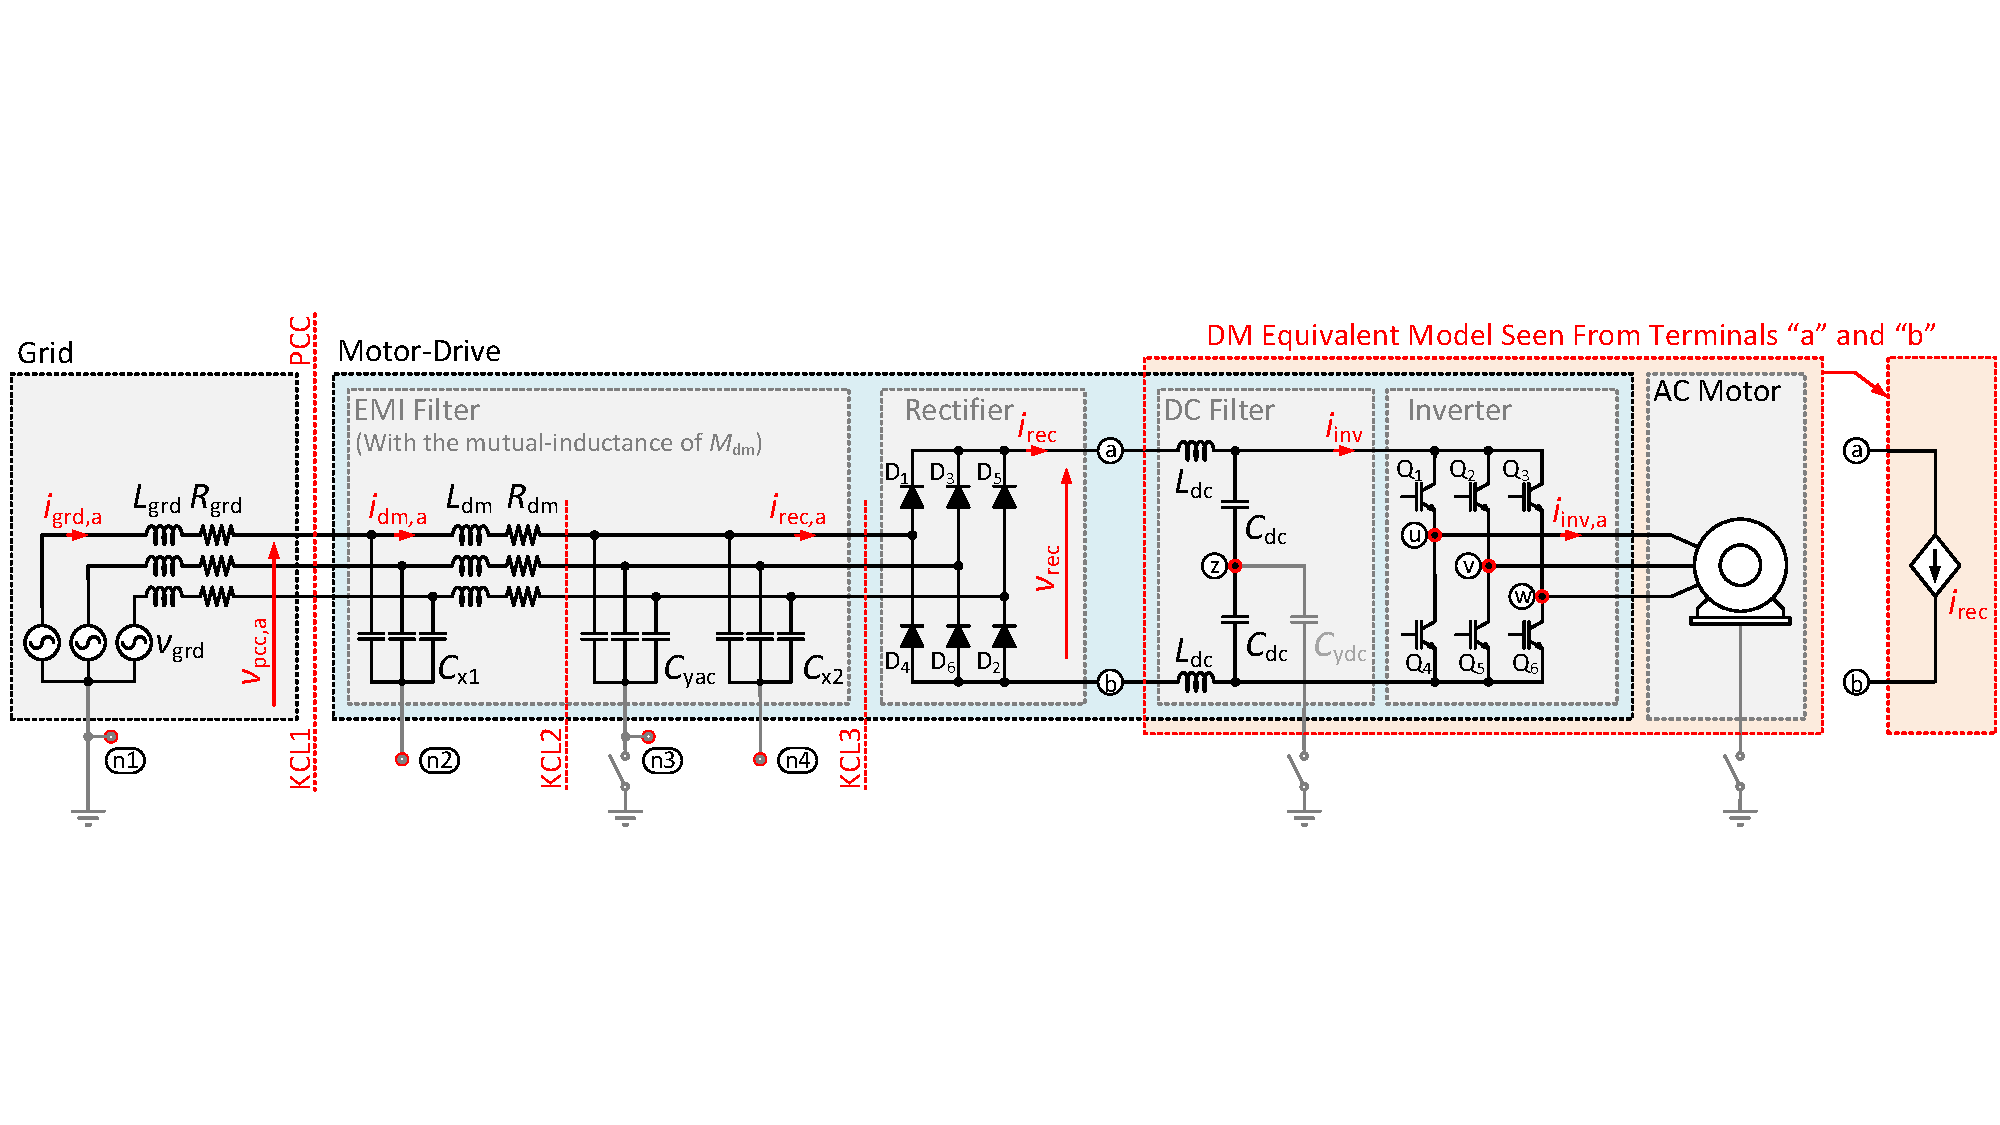
\includegraphics[clip, trim=0cm 5cm 0cm 5cm, width=1\linewidth]{FIGS/FIG_1.pdf}
			    \caption{The motor-drive system under study for common-mode EMI investigations.}
			    \label{FIG1}
			    \vspace{-5mm}
	    \end{figure*}
		
		%%EQ1
		\begin{flalign}
	        i_{\mathrm{inv}}(t)=\sum\limits_{x{\in}{\mathrm{a,b,c}}}s_{\mathrm{inv},x}(t)i_{\mathrm{inv},x}(t) &&
	        \label{EQ1}
	    \end{flalign}
	    
	    %%EQ2
		\begin{flalign}
	        I_{\mathrm{inv}}=\sum\limits_{x{\in}{\mathrm{a,b,c}}}S_{\mathrm{inv},x}\ast I_{\mathrm{inv},x} &&
	        \label{EQ2}
	    \end{flalign}
		
		{\color{red}This equation~needs further discussion $\downarrow$
		
		%%EQ3
		\begin{flalign}
	        I_{\mathrm{rec}}=
	        \underbrace{\frac{1}{(Z_\mathrm{L,dc}+Z_\mathrm{C,dc})}}_{Y_\mathrm{dc}}
	        V_{\mathrm{rec}}+
	        \underbrace{\frac{Z_\mathrm{C,dc}}{(Z_\mathrm{L,dc}+Z_\mathrm{C,dc})}}_{H_\mathrm{dc}}
	        I_\mathrm{inv} &&
	        \label{EQ3}
	    \end{flalign}
		}
		%%FIG2
		\begin{figure}[t]
			    \centering
			    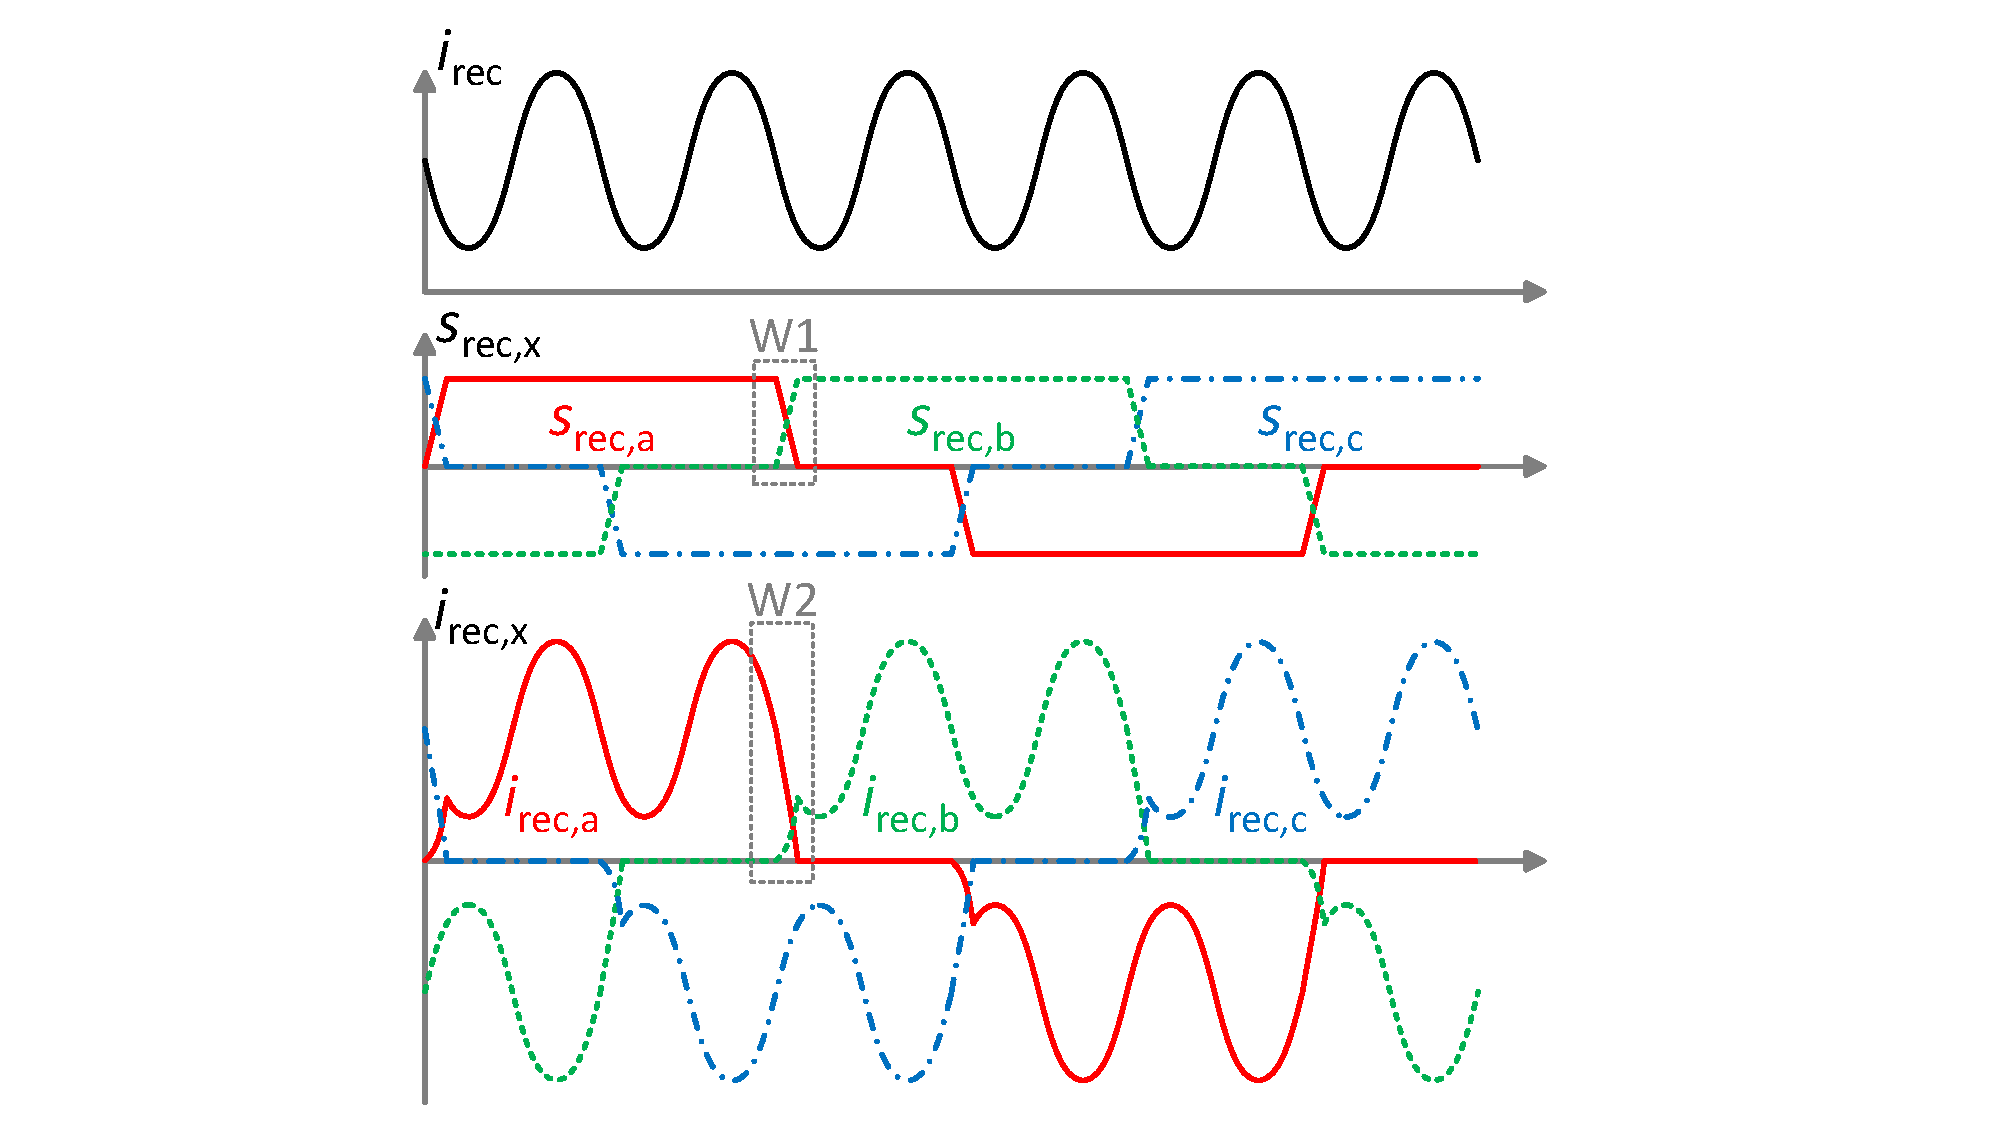
\includegraphics[clip, trim=5cm 0cm 5cm 0cm, width=1\linewidth]{FIGS/FIG_2.pdf}
			    \caption{Reconstruction of the rectifier input currents with its output current and its switching pattern.
			    {\color{red}\{Modes of operation should be highlighted somewhere in the figure\}.}}
			    \label{FIG2}
			    \vspace{-7}
	    \end{figure}
		
		%%FIG3
		\begin{figure}[t]
			    \centering
			    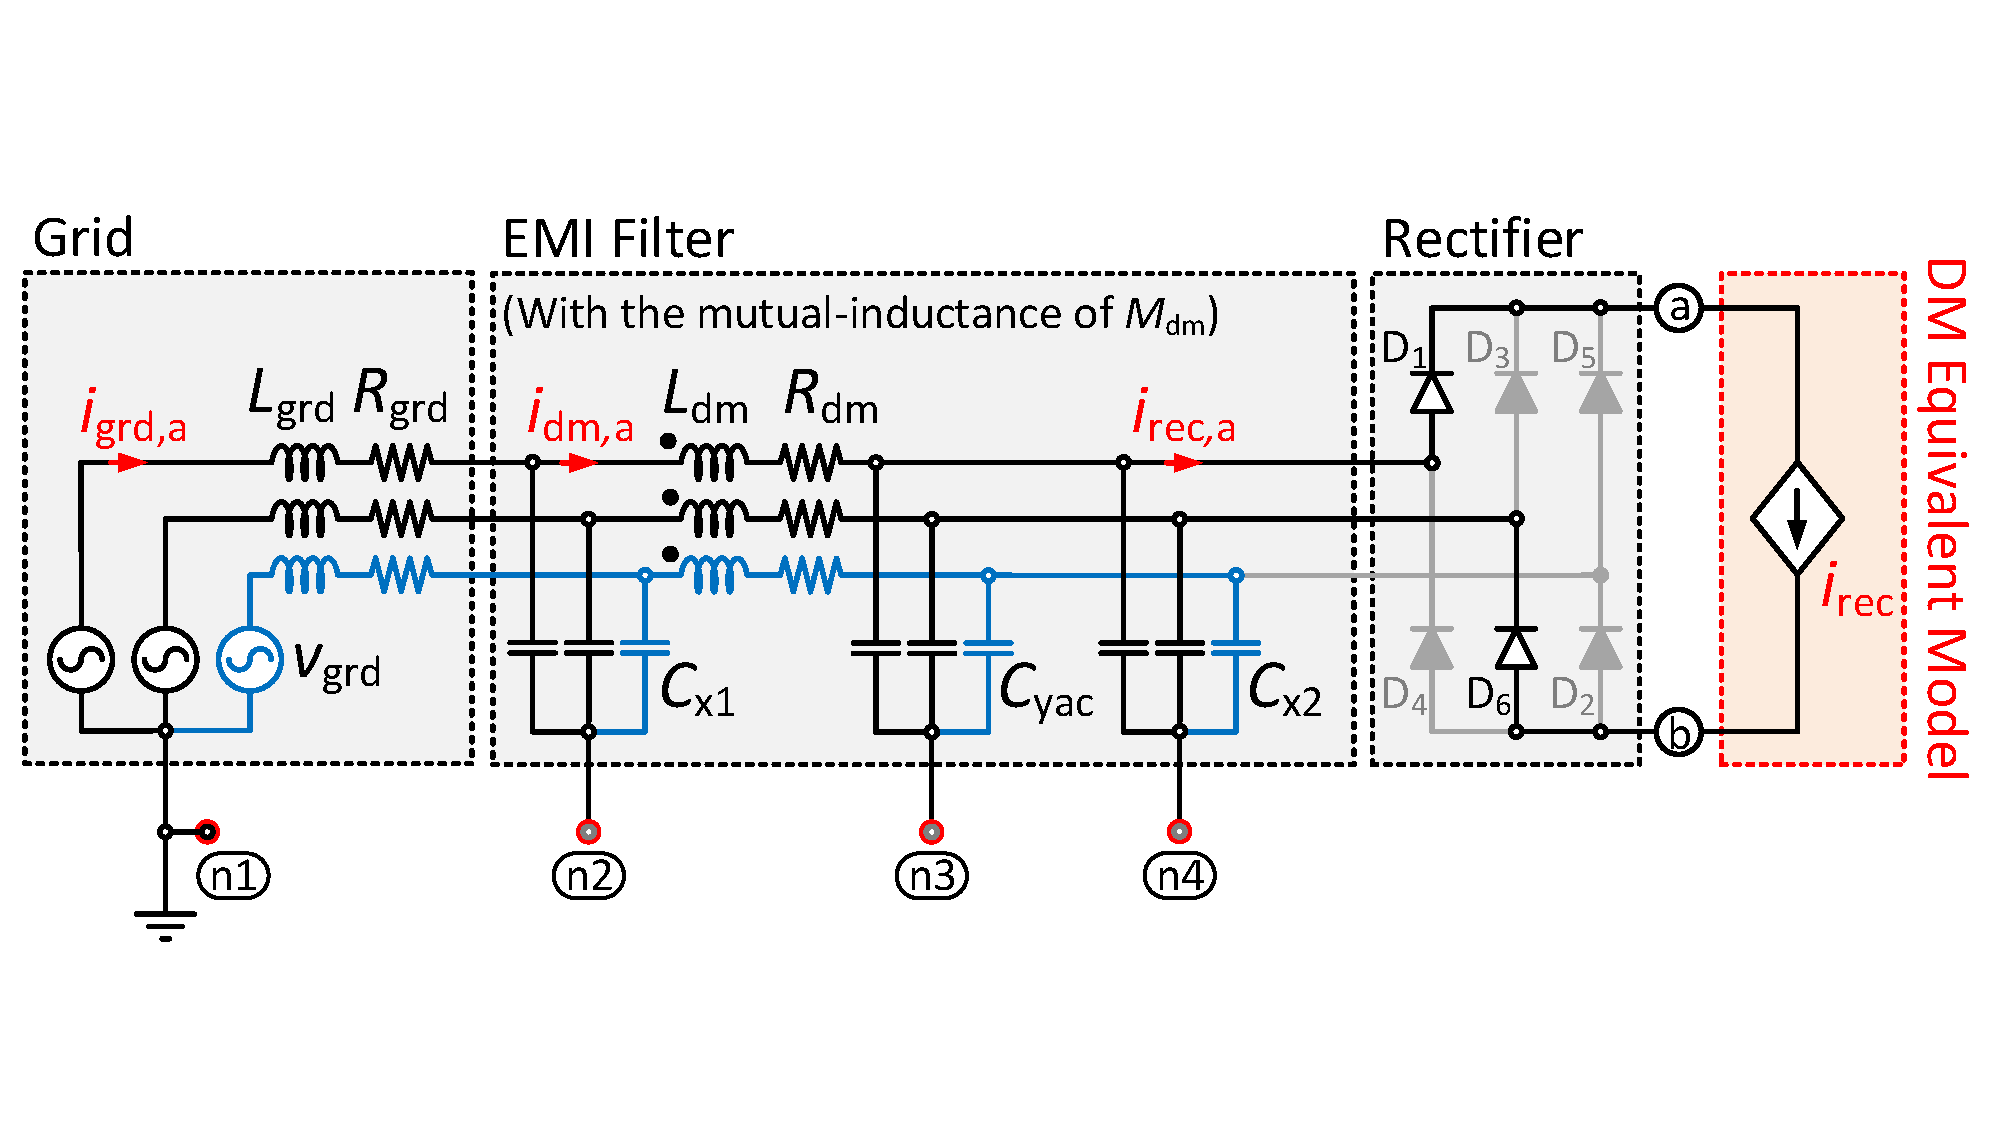
\includegraphics[clip, trim=0cm 3cm 0cm 3cm, width=1\linewidth]{FIGS/FIG_3.pdf}
			    \caption{Conduction of DM current in the motor-drive system shown in Fig.~\ref{FIG1}. {\color{red}\{Mode of operation should be highlighted somewhere in the figure\}.}
			    {\color{red}\{With LISN the level of mode-changing transients (DM EMI) is significantly reduced (We only have the experimental results for the case with LISN)\}.}}
			    \label{FIG3}
	    \end{figure}
		
		%%FIG4
		\begin{figure}[t]
	        \centering
	   %     \subfloat[]{
		  %      \includegraphics[clip, trim=1.25cm 6.5cm 1.25cm 7cm, width=1\linewidth]{FIGS/FIG_4A.eps}
		  %  }\\
		  %  \vspace{-3mm}
		  %  \subfloat[]{
		        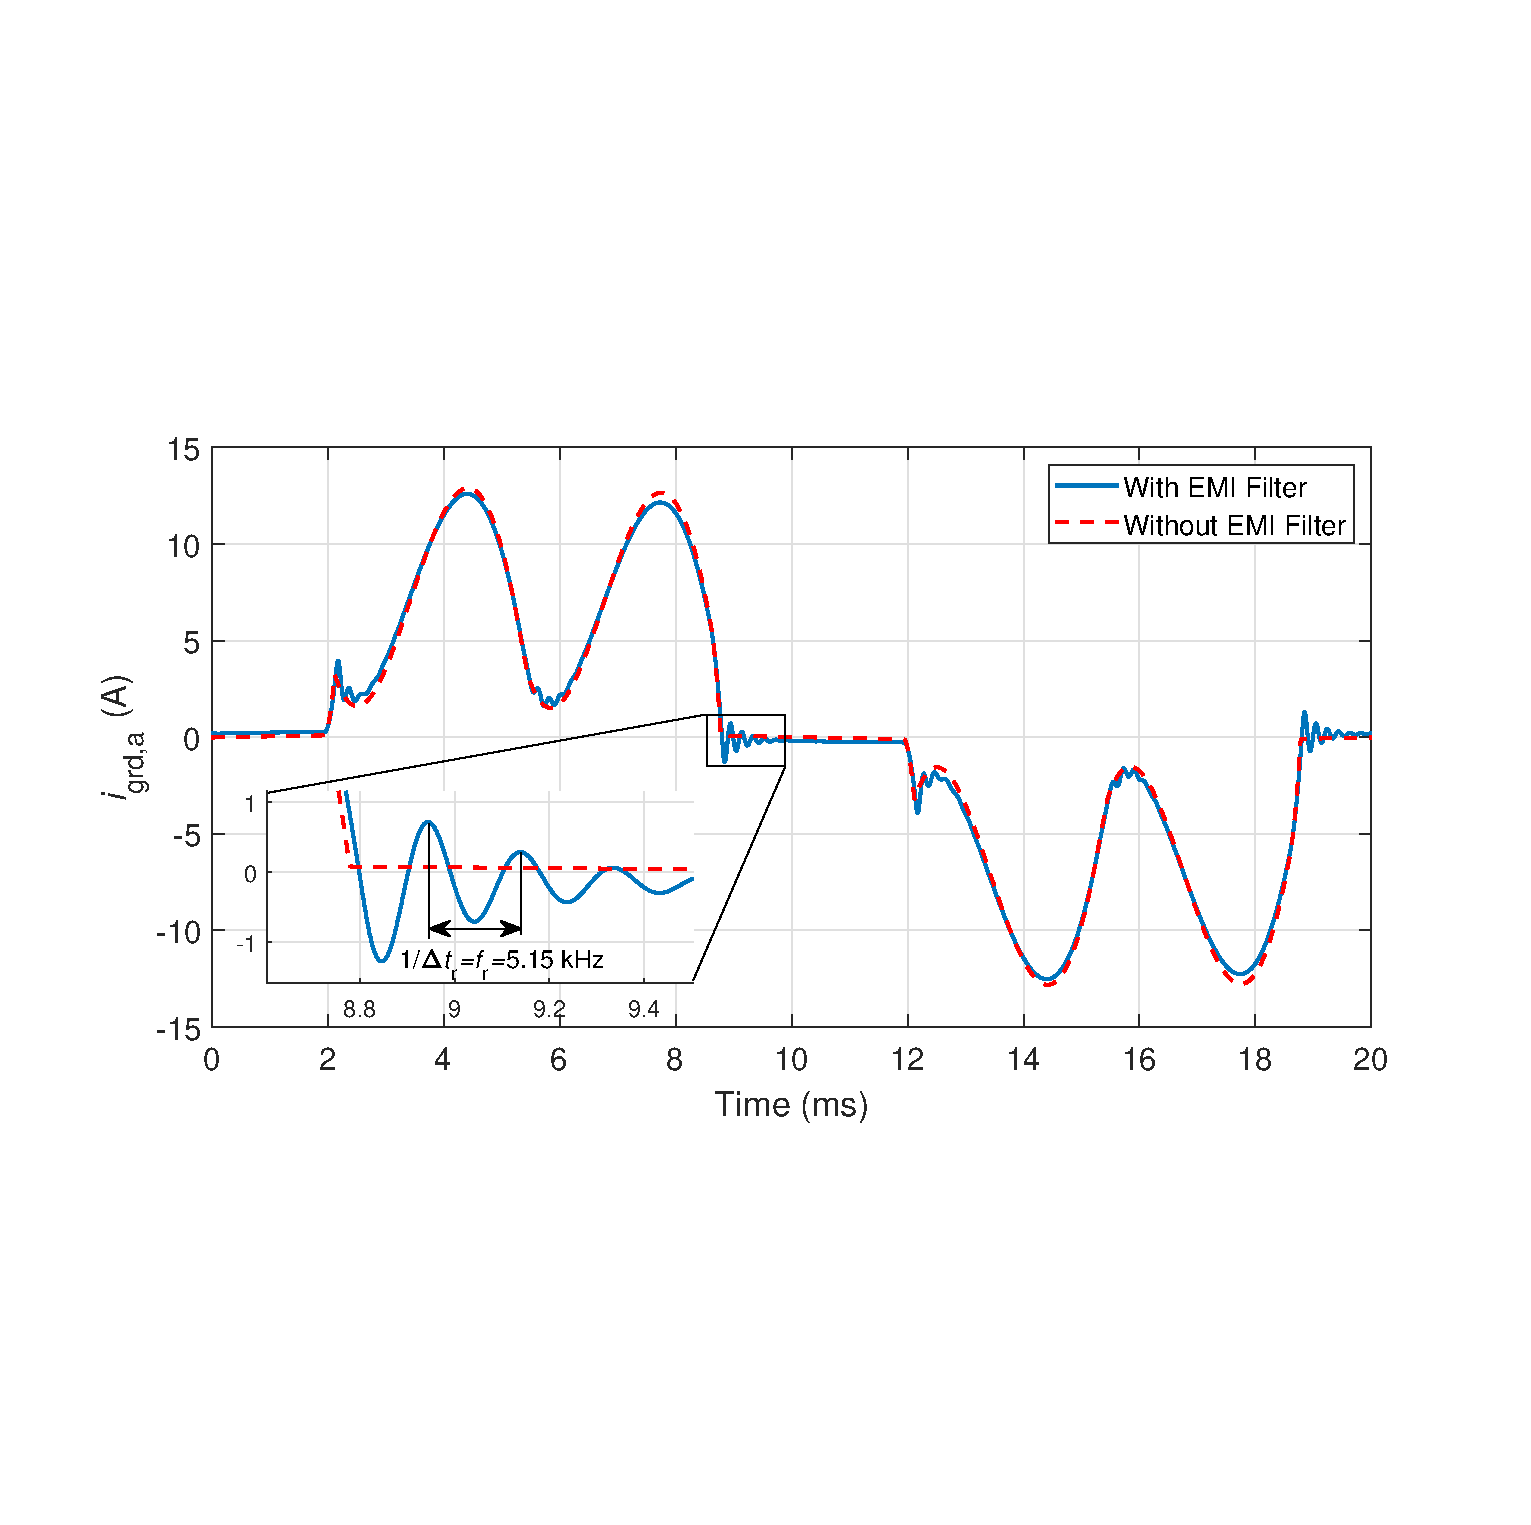
\includegraphics[clip, trim=1.25cm 6.5cm 1.25cm 7cm, width=1\linewidth]{FIGS/FIG_4.eps}
		  %  }
		    %\caption{Time-domain results for (a) the grid current $i_{\mathrm{grd,a}}$ and (b) PCC voltage $v_{\mathrm{pcc,a}}$ of the motor-drive system when it is equipped and not equipped with EMI filter. {\color{red}\{Modes of operation should be highlighted somewhere in the figure\}.}}
		    \caption{Time-domain results for the grid current $i_{\mathrm{grd,a}}$ of the motor-drive system when it is equipped and not equipped with EMI filter. {\color{red}\{Modes of operation should be highlighted somewhere in the figure\}.}}
		    \label{FIG11}
	    \end{figure}

		%%FIG5
		\begin{figure}[h!]
			    \centering
			    \subfloat[]{
	                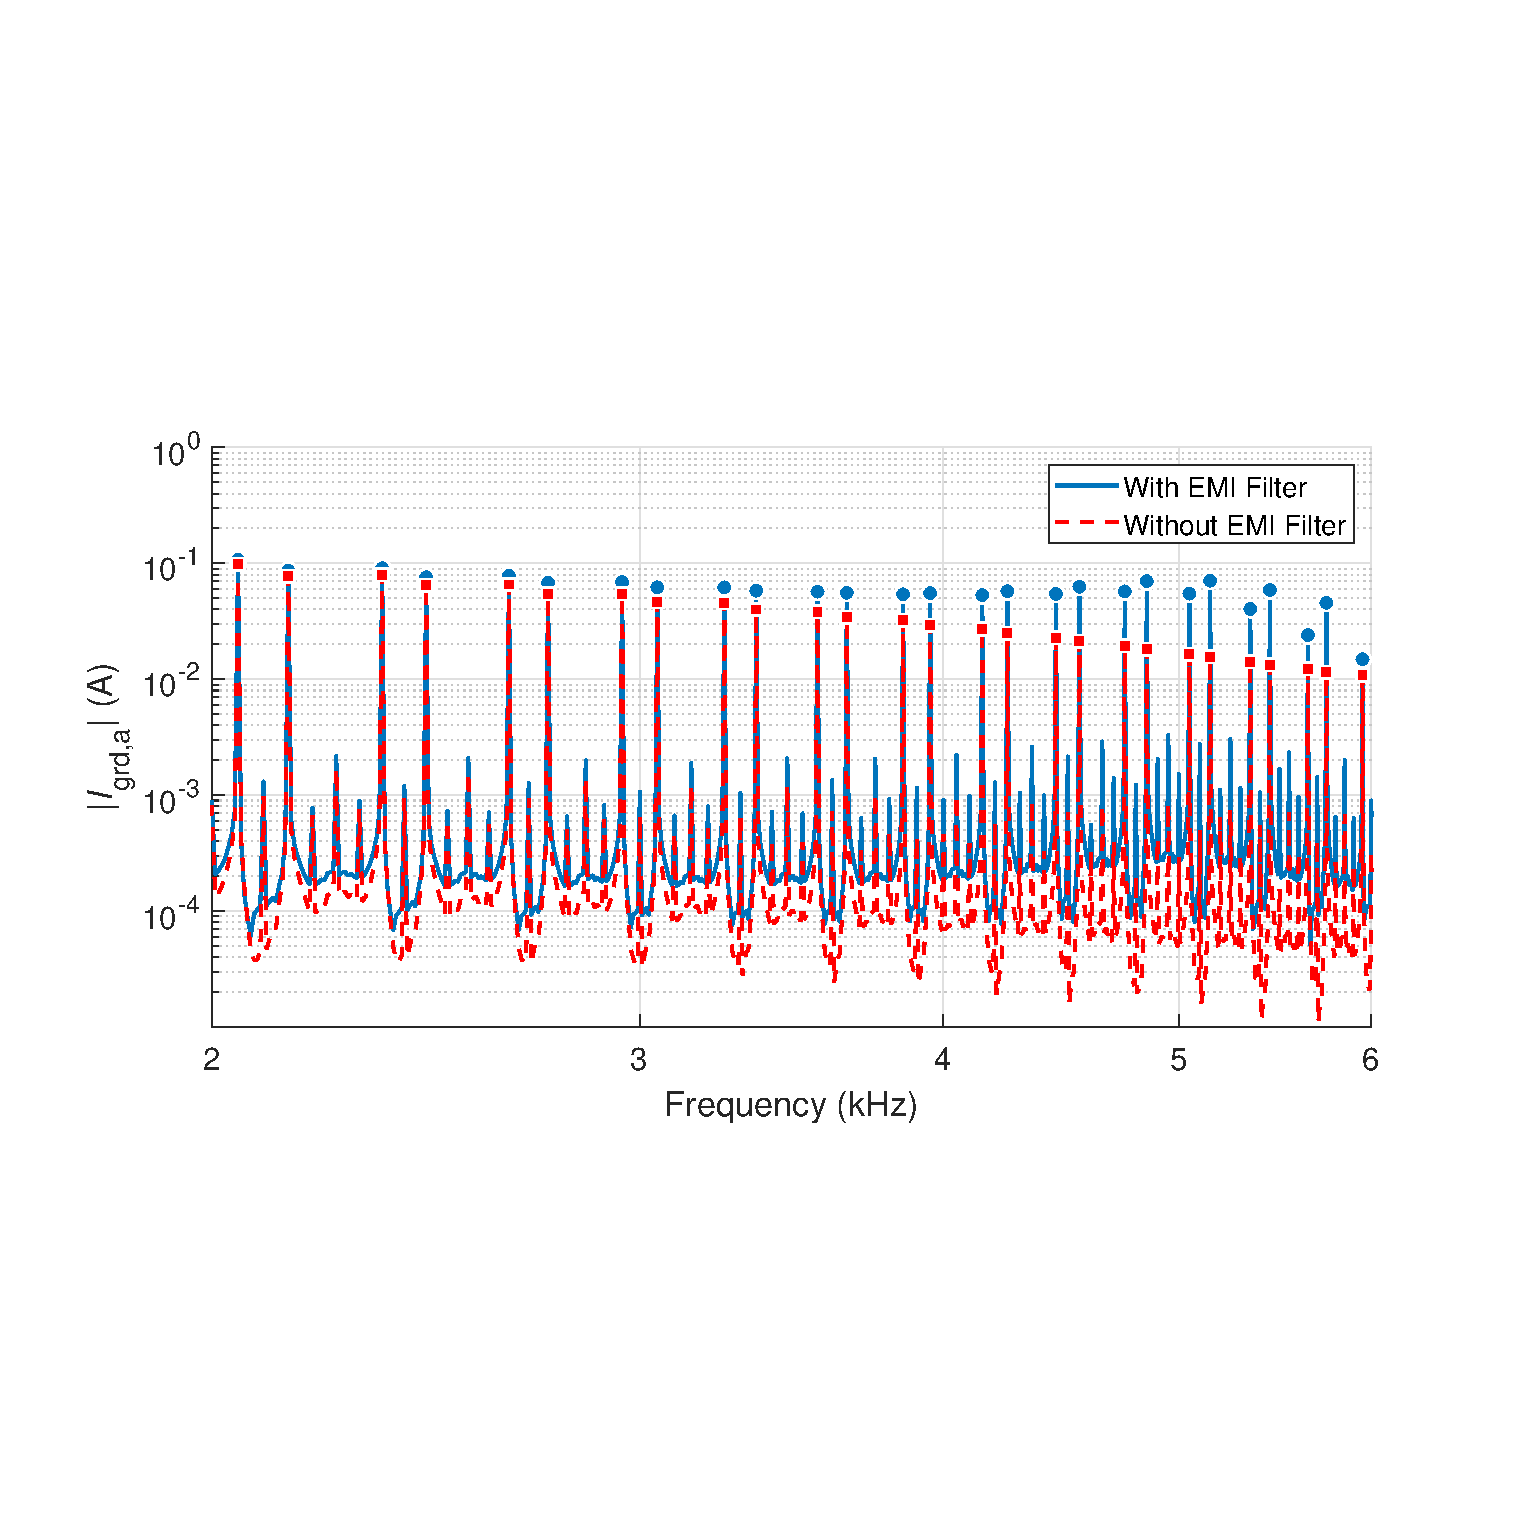
\includegraphics[clip, trim=1.25cm 6.5cm 1.25cm 7cm, width=1\linewidth]{FIGS/FIG_5A.eps}
	                }\\ \vspace{-3mm}
	            \subfloat[]{
	                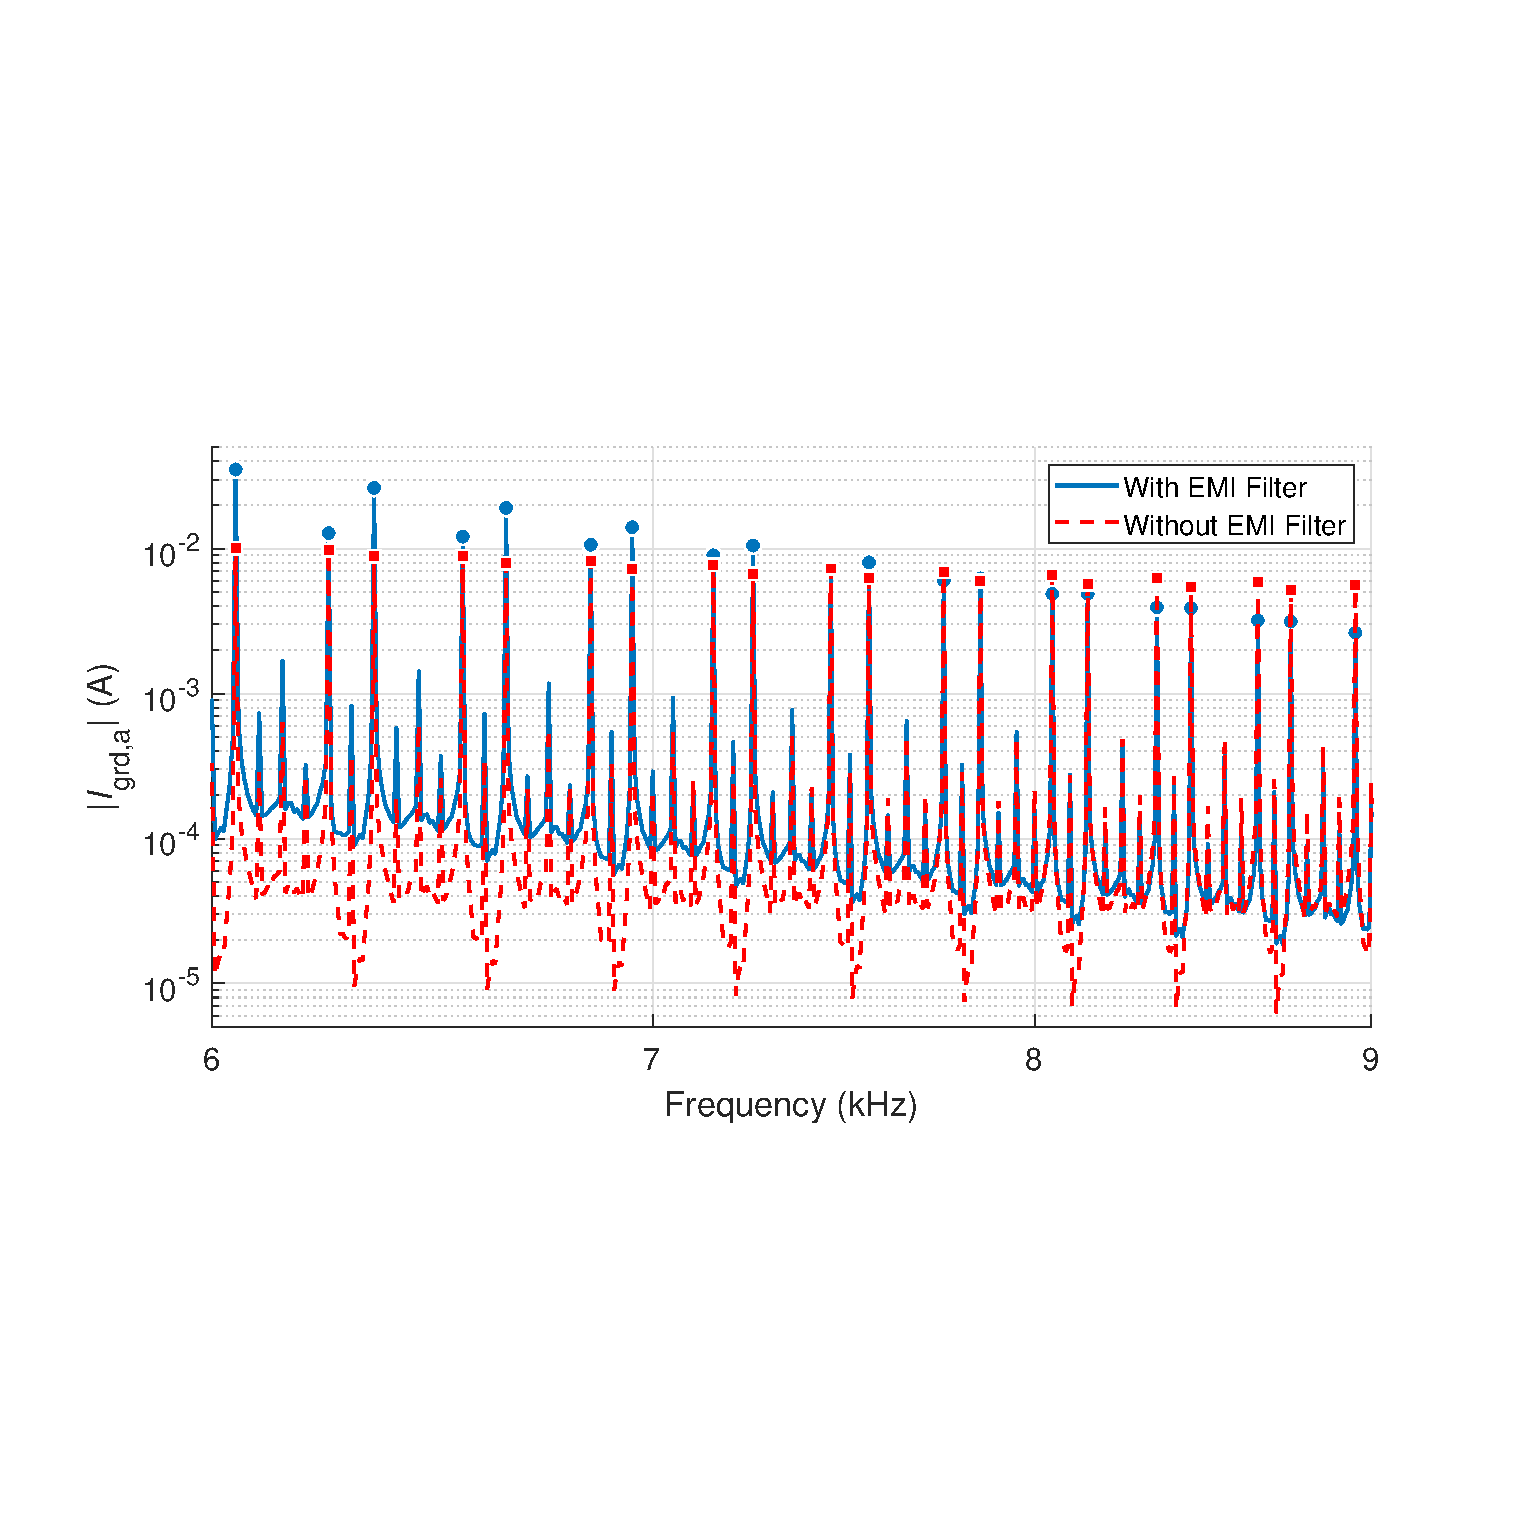
\includegraphics[clip, trim=1.25cm 6.5cm 1.25cm 7cm, width=1\linewidth]{FIGS/FIG_5B.eps}
	            }
			    \caption{Frequency-domain results for the  grid current ($|I_\mathrm{grd,a}|$) of the motor-drive system EMI filter with EMI filter (solid blue line with circular blue markers) and without EMI filter (red dashed line with squared red markers) for (a) 2-6 kHz and (b) 6-9 kHz.} 
			    \label{FIG5}
	    \end{figure}
		
		\noindent where $Z_{\mathrm{C,dc}}=-\mathrm{j}2/\left(\omega C_{\mathrm{dc}}\right)$ and $Z_{\mathrm{L,dc}}=\mathrm{j}2\omega L_\mathrm{L,dc}$.
		
		{\color{red} As it can be seen in \eqref{EQ3}, the rectifier output current $i_\mathrm{rec}$ can be influenced by both the inverter EMI, through $Y_{\mathrm{dc}}$, and its output voltage ($v_\mathrm{rec}$) EMI, through $H_\mathrm{dc}$.}
		
		Finally, as it is shown in Fig.~\ref{FIG2}, the output current of the rectifier $i_\mathrm{rec}$ is dispersed into its input currents $i_{\mathrm{rec},x}$ through its switching pattern $s_{\mathrm{rec},x}$. Therefore, $i_{\mathrm{rec}}$ can be obtained as in \eqref{EQ4} in time-domain. The resultant frequency-domain relationship of $i_\mathrm{rec}$ can be written as \eqref{EQ5}.
		
		%%EQ4
		\begin{flalign}
	        i_{\mathrm{rec},x}(t)=s_{\mathrm{rec},x}(t)i_\mathrm{rec}(t) &&
	        \label{EQ4}
	    \end{flalign}
		
		%%EQ5
		\begin{flalign}
	        I_{\mathrm{rec},x}=S_{\mathrm{rec,x}}\ast I_{\mathrm{inv},x} &&
	        \label{EQ5}
	    \end{flalign}

	\section{Effect of EMI filter on the Propagation of DM Noises Caused by the diode Rectifier}
	
	In this section, the effect of EMI filter on the DM noises generated by the diode rectifier is investigated. Fig.~\ref{FIG3} shows a more simplified representation of Fig.~\ref{FIG1}, in which how EMI filter is involved in the DM noise propagation (when $\mathrm{D}_1$ and $\mathrm{D}_6$ are ON) is shown. The highlighted rectifier mode (shaded in black) in Fig.~\ref{FIG1} lasts for $60^\circ$, and it is one of the main six modes of operation in a rectifier to form the six-pulse output rectified current $i_\mathrm{rec}$ shown in Fig.~\ref{FIG2}. Transition from one mode to the other (mode-changing transients) (e.g. ($\mathrm{D}_6,\mathrm{D}_1$: ON) to ($\mathrm{D}_1,\mathrm{D}_2$: ON)) ends up with some transients that can resonate with the EMI filter and the grid impedance. These transients, therefore, can be intensified by the EMI filter, and they can leak through the EMI filter to the grid-side more effectively. 
	
	To study how the interaction of the EMI filter and the grid impedance affects the leakage of DM noises produced by the rectifier to the grid-side, the system shown in Fig.~\ref{FIG1} is studied with and without EMI filter. For this purpose, the system is numerically modelled in MATLAB/Simulink {\color{red}and experimentally tested} based on the specifications given in TABLE~\ref{TBL1}. This system is a $100~\mathrm{kVA}$, $415~\mathrm{V}$ distribution network with a stiff grid impedance of $Z_{\mathrm{grd}}=Z_\mathrm{grd,0}$ (which is less than $1.8\%$ of the feeder and transformer base impedance $Z_{\mathrm{b}}=1.72~\Omega$). Figs.~\ref{FIG4} and \ref{FIG5} show the obtained time-domain and frequency-domain results for the grid current $i_{\mathrm{grd,a}}$ with and without EMI filter, respectively.
	
	%% TBL1
	 \begin{table} [b]
	    \begin{center}
	    \caption{Specifications of the motor-drive system. {\color{red}\{(1) Do we need to specifically mention the DC link parameters (they are all neglected by considering the drive system as current sources)? (Resistance of the DC coil is not included.) (2) $R_\mathrm{g}$ and $L_\mathrm{g}$ should be changed to $R_\mathrm{grd}$ and $L_\mathrm{grd}$.\}}}
	    \vspace{-2mm}
	    \label{TBL1}
	            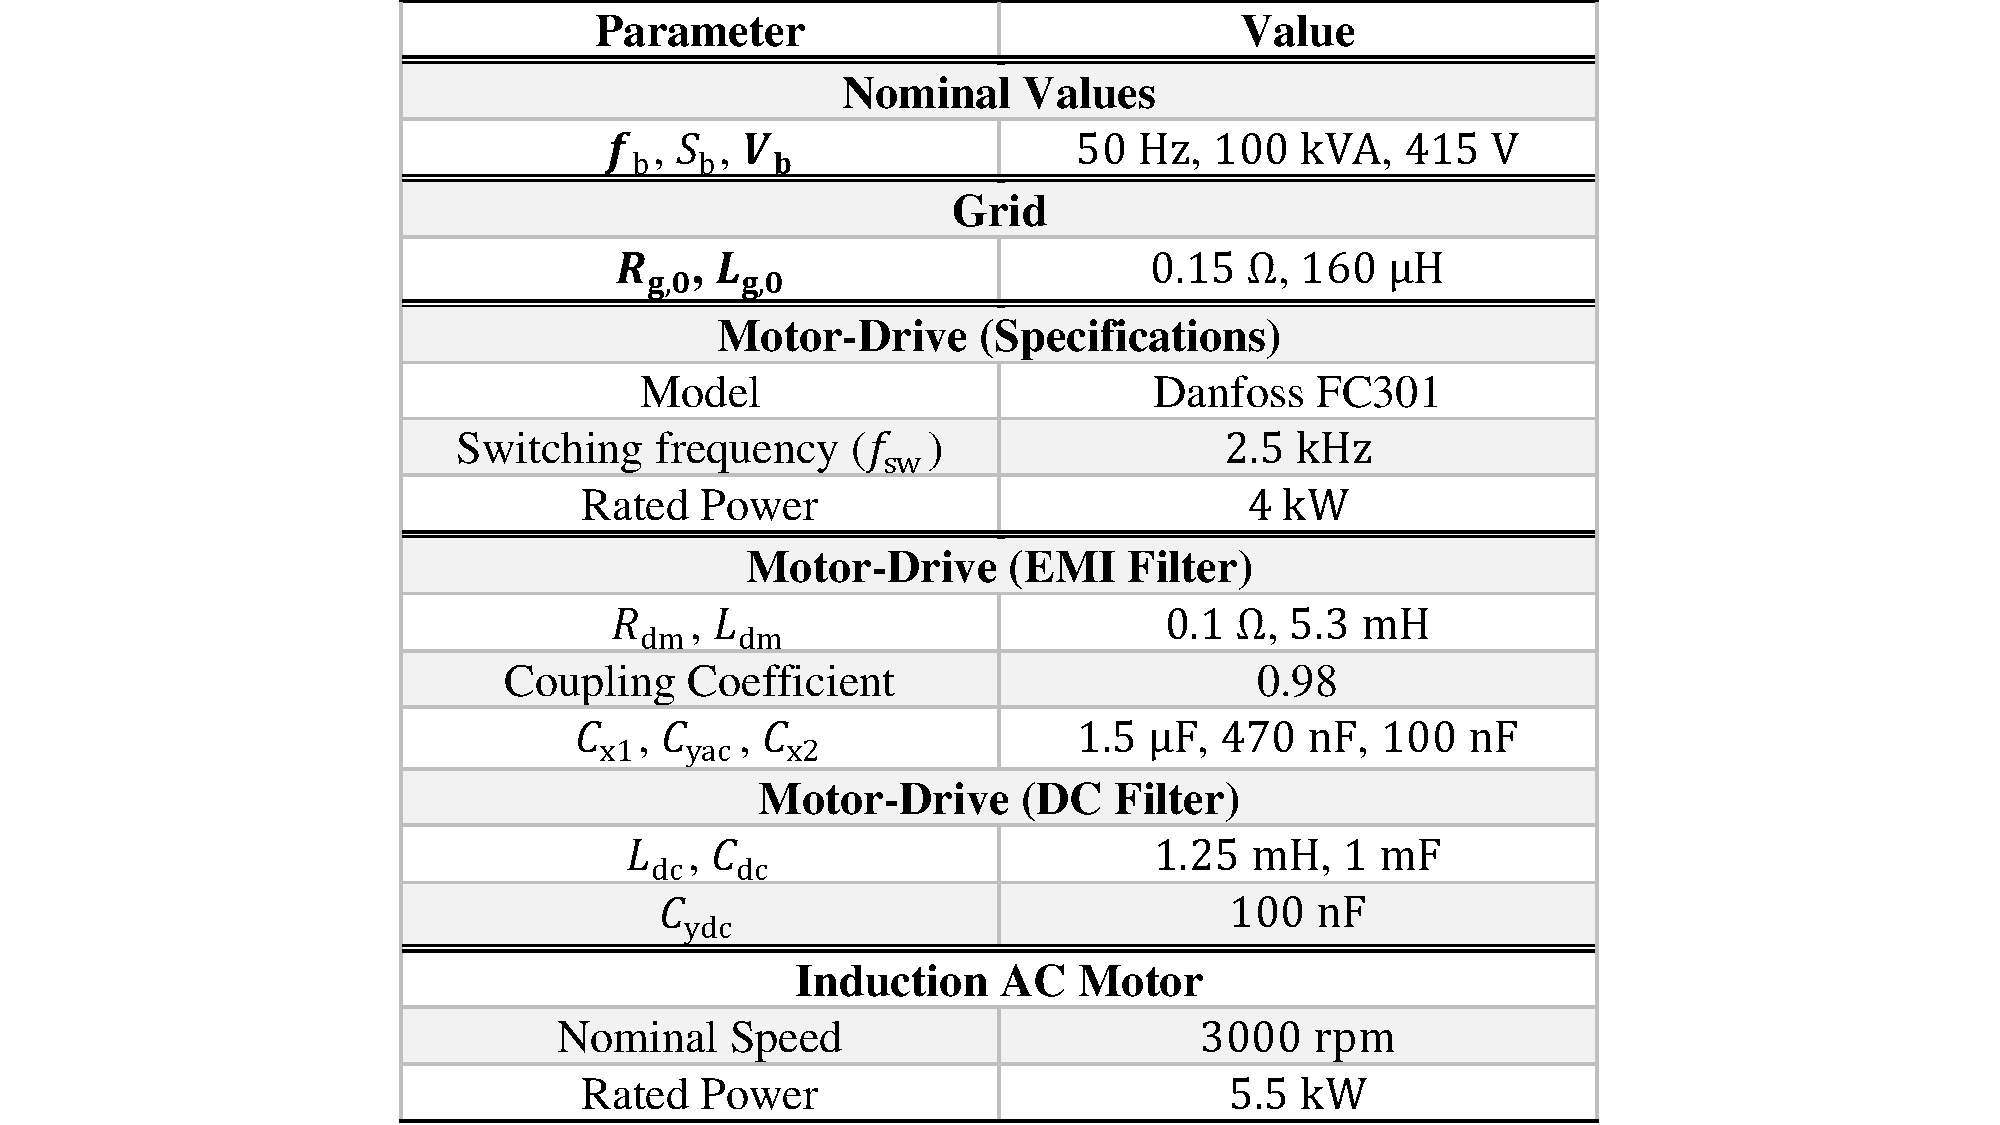
\includegraphics[clip, trim=65mm 0mm 65mm 0mm, width=1\columnwidth]{FIGS/TBL_1.pdf}
	    \end{center}
	    \vspace{-3mm}
	\end{table}
	
	%For each case, two different types of a stiff grid ($Z_{\mathrm{grd}}=Z_\mathrm{grd,0}$ which less than $1.8\%$ of the feeder and transformer base impedance $Z_{\mathrm{b}}=1.72~\Omega$) and a week grid ($Z_{\mathrm{grd}}=10\times Z_\mathrm{grd,0}$, which is more than $18.2\%$ of $Z_{\mathrm{b}}$) is considered. Fig.~\ref{}
	
	%For the stiff grid, $Z_{\mathrm{grd}}=Z_\mathrm{grd,0}$ and for the weak grid .
	As it can be seen in time-domain and frequency-domain results shown in Figs.~\ref{FIG4} and \ref{FIG5}, in contrast to what EMI filter is designed for, it can conduct more DM EMI noises compared to the case without EMI filter. In the time-domain results shown in Fig.~\ref{FIG4} for the case without EMI (solid black line), these noises appear at the moment of transitions and in the form of ringings. {\color{gray}\{In this figure, each mode and its on-state diodes are highlighted in its respective regions.\}}. This is while the level of transients for the case without EMI filter is significantly smaller. This phenomenon can also be seen in the frequency contents shown in Fig.~\ref{FIG5}. As it can be seen in this figure, when the rectifier is equipped with an EMI filter, the level of noises can remarkably increases from the case without EMI filter at a certain range of frequencies (around $5.15~\mathrm{kHz}$). In the next section, the mode-changing transients caused by the operation of the rectifier in the proposed motor-drive system is further investigated.
	
	%%FIG6
	\begin{figure}[t]
	    \centering
		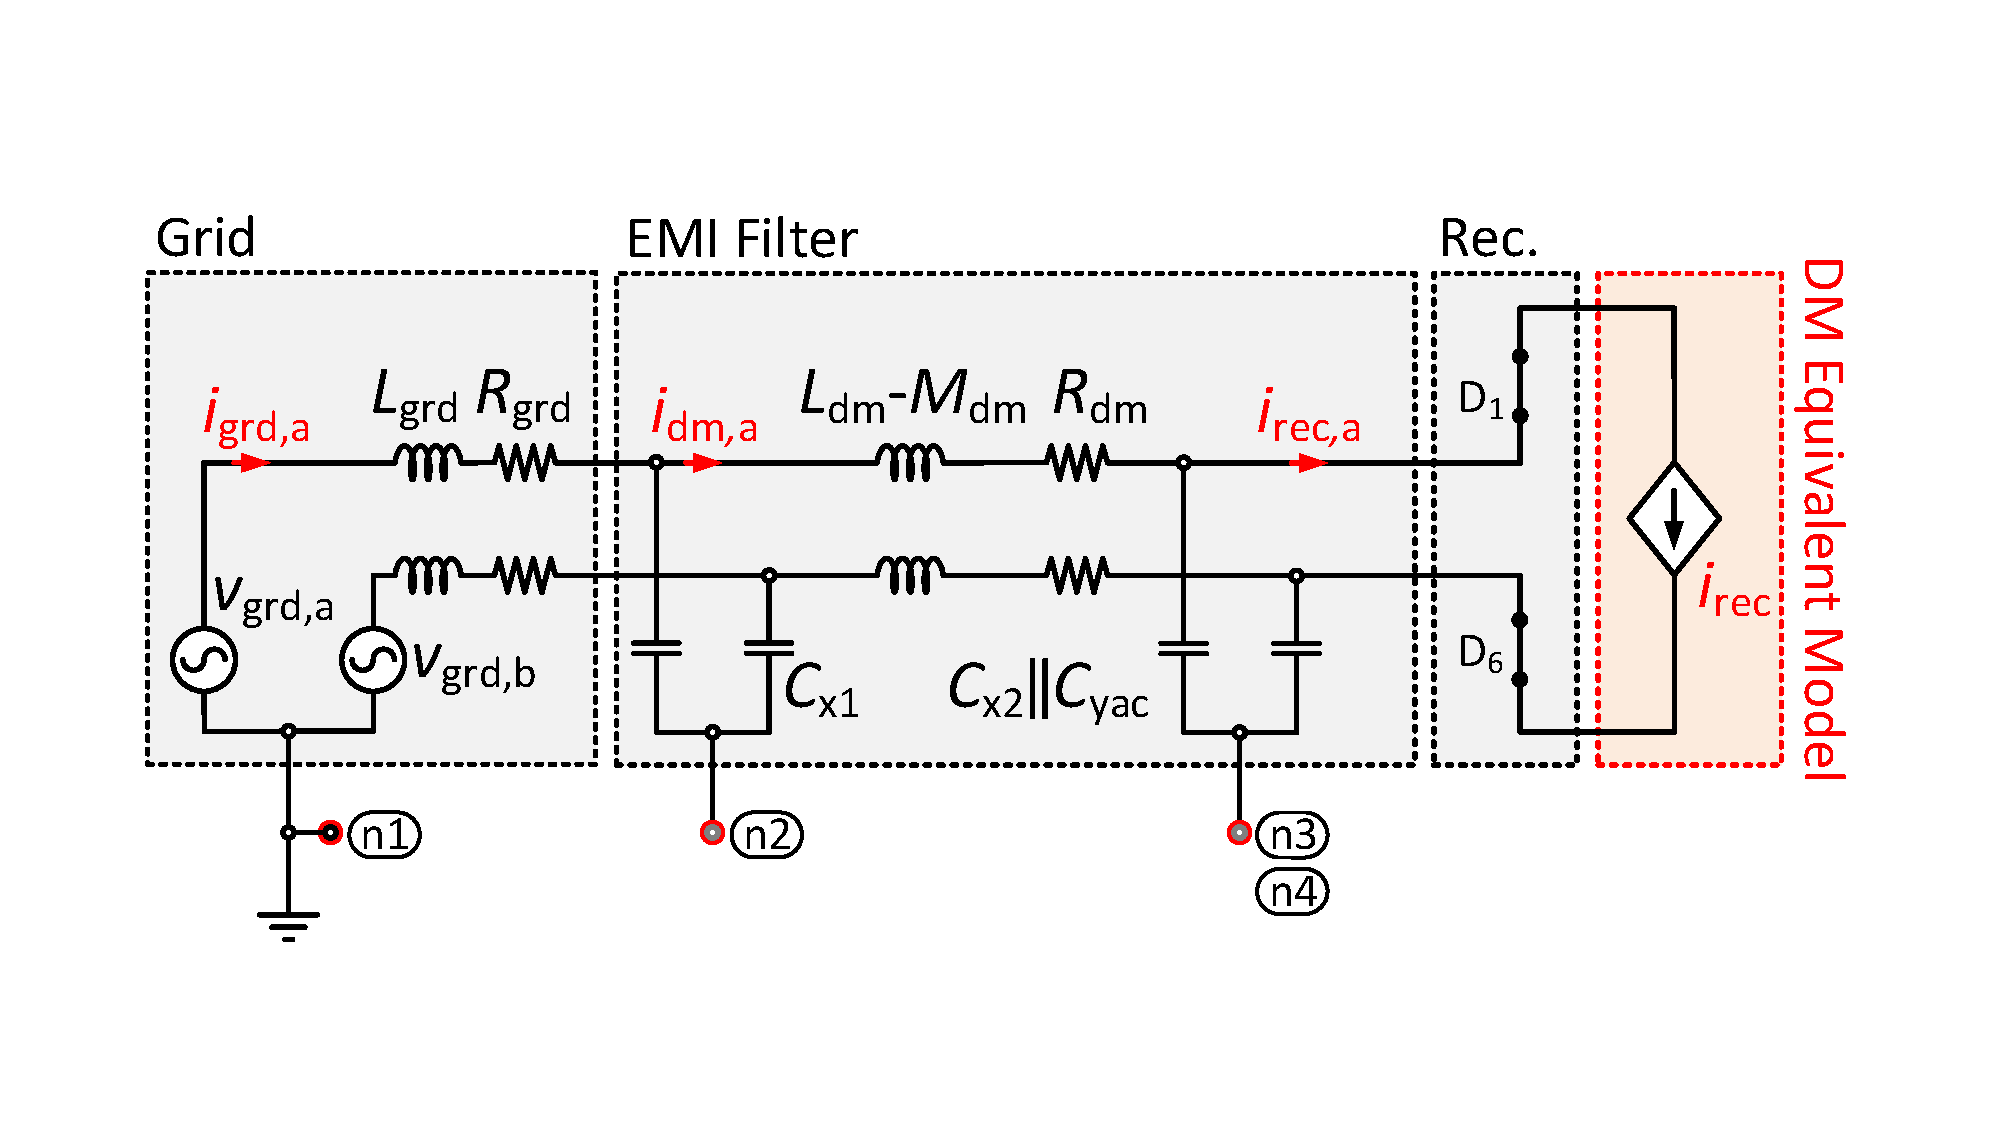
\includegraphics[clip, trim=0cm 3cm 0cm 3cm, width=1\linewidth]{FIGS/FIG_6.pdf}
		\caption{Two-phase equivalent circuit to analyze DM EMI in the motor-drive system shown in Fig.~\ref{FIG1}. {\color{red}\{I should carefully think about the phase instances.\}}{\color{blue}\{Do we have any reference for it?\}}}
		\label{FIG6}
	\end{figure}
	
	%%FIG7
    \begin{figure}
	    \begin{center}
	        \subfloat[]{
	                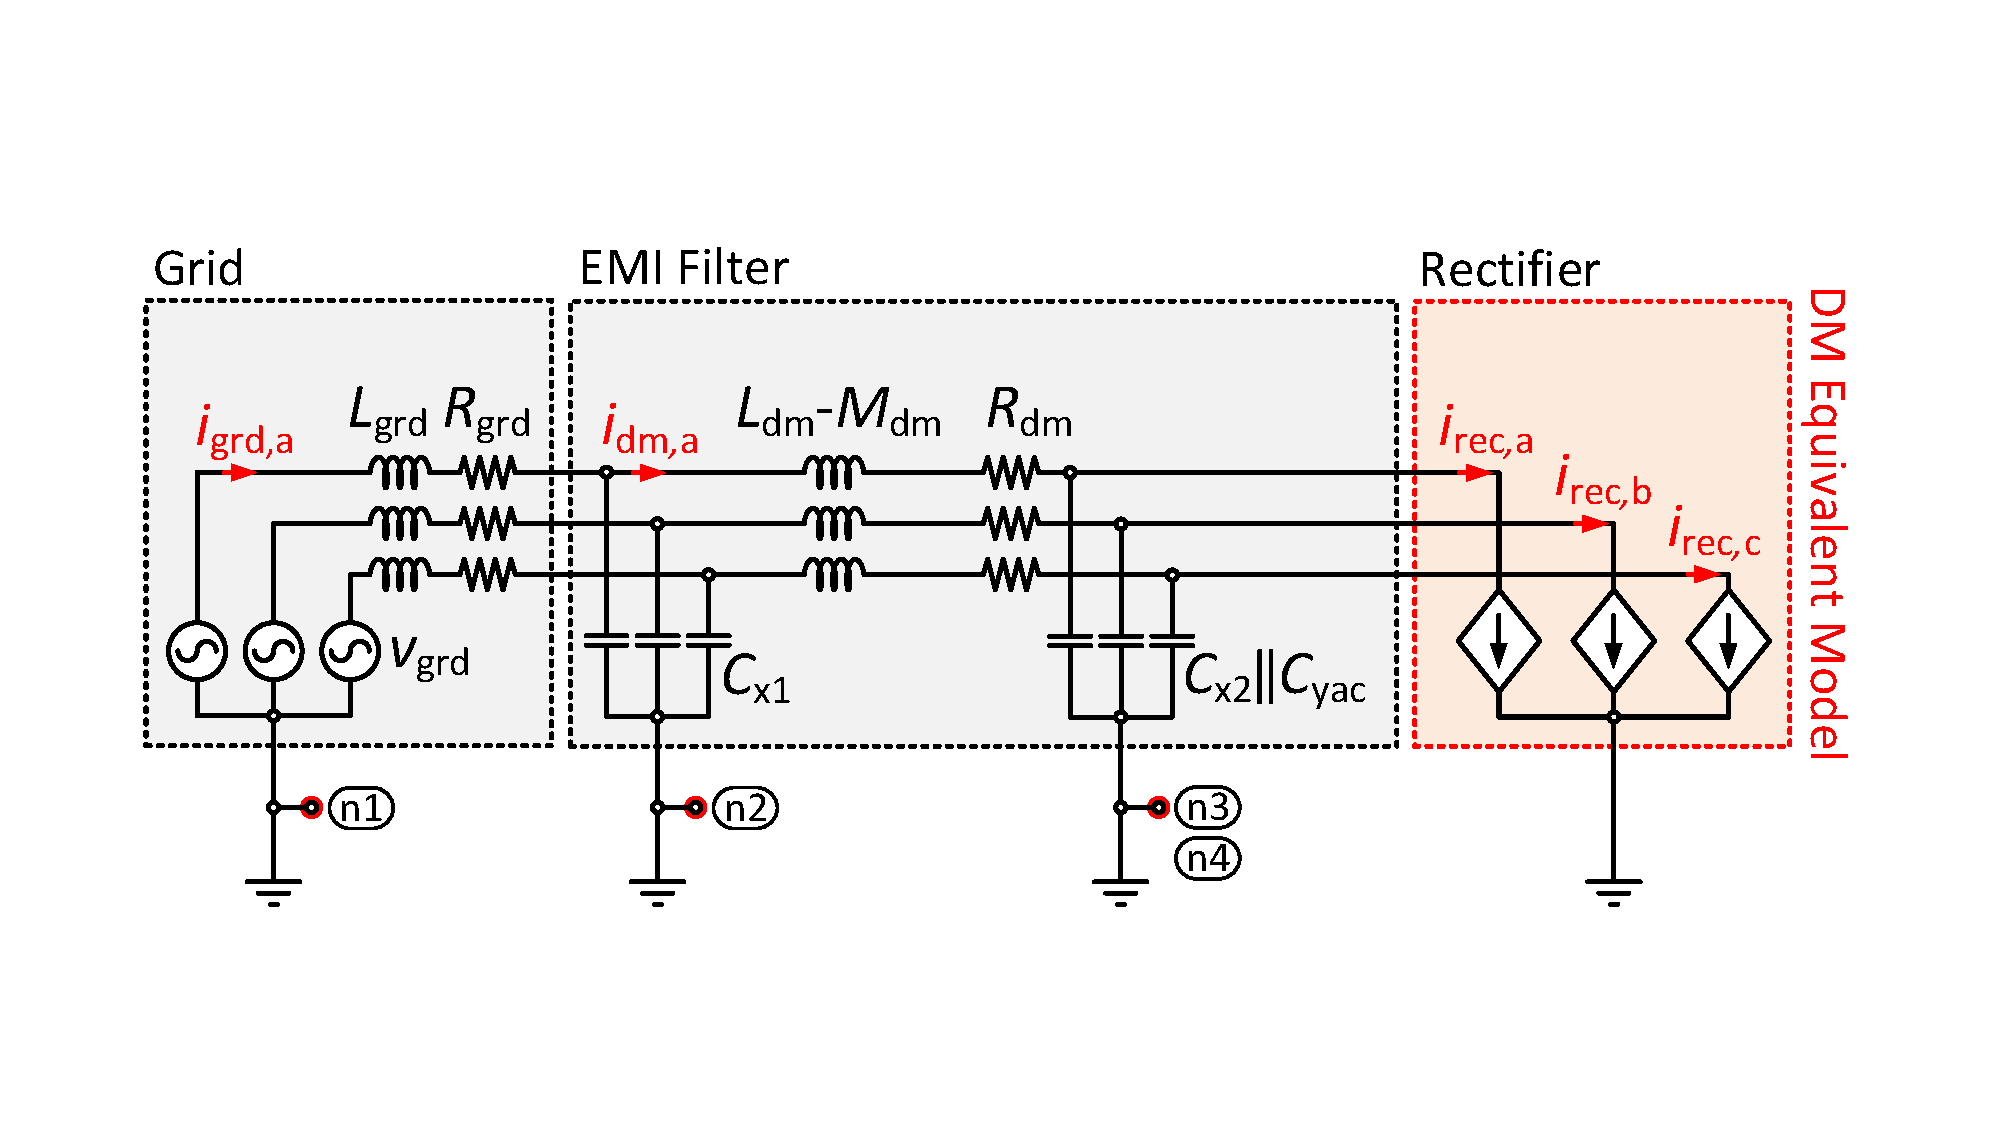
\includegraphics[clip, trim=2.25cm 3cm 2.25cm 3cm, width=1\linewidth]{FIGS/FIG_7A.pdf}
	                }
	                \\
	                \vspace{-3mm}
	        \subfloat[]{
	                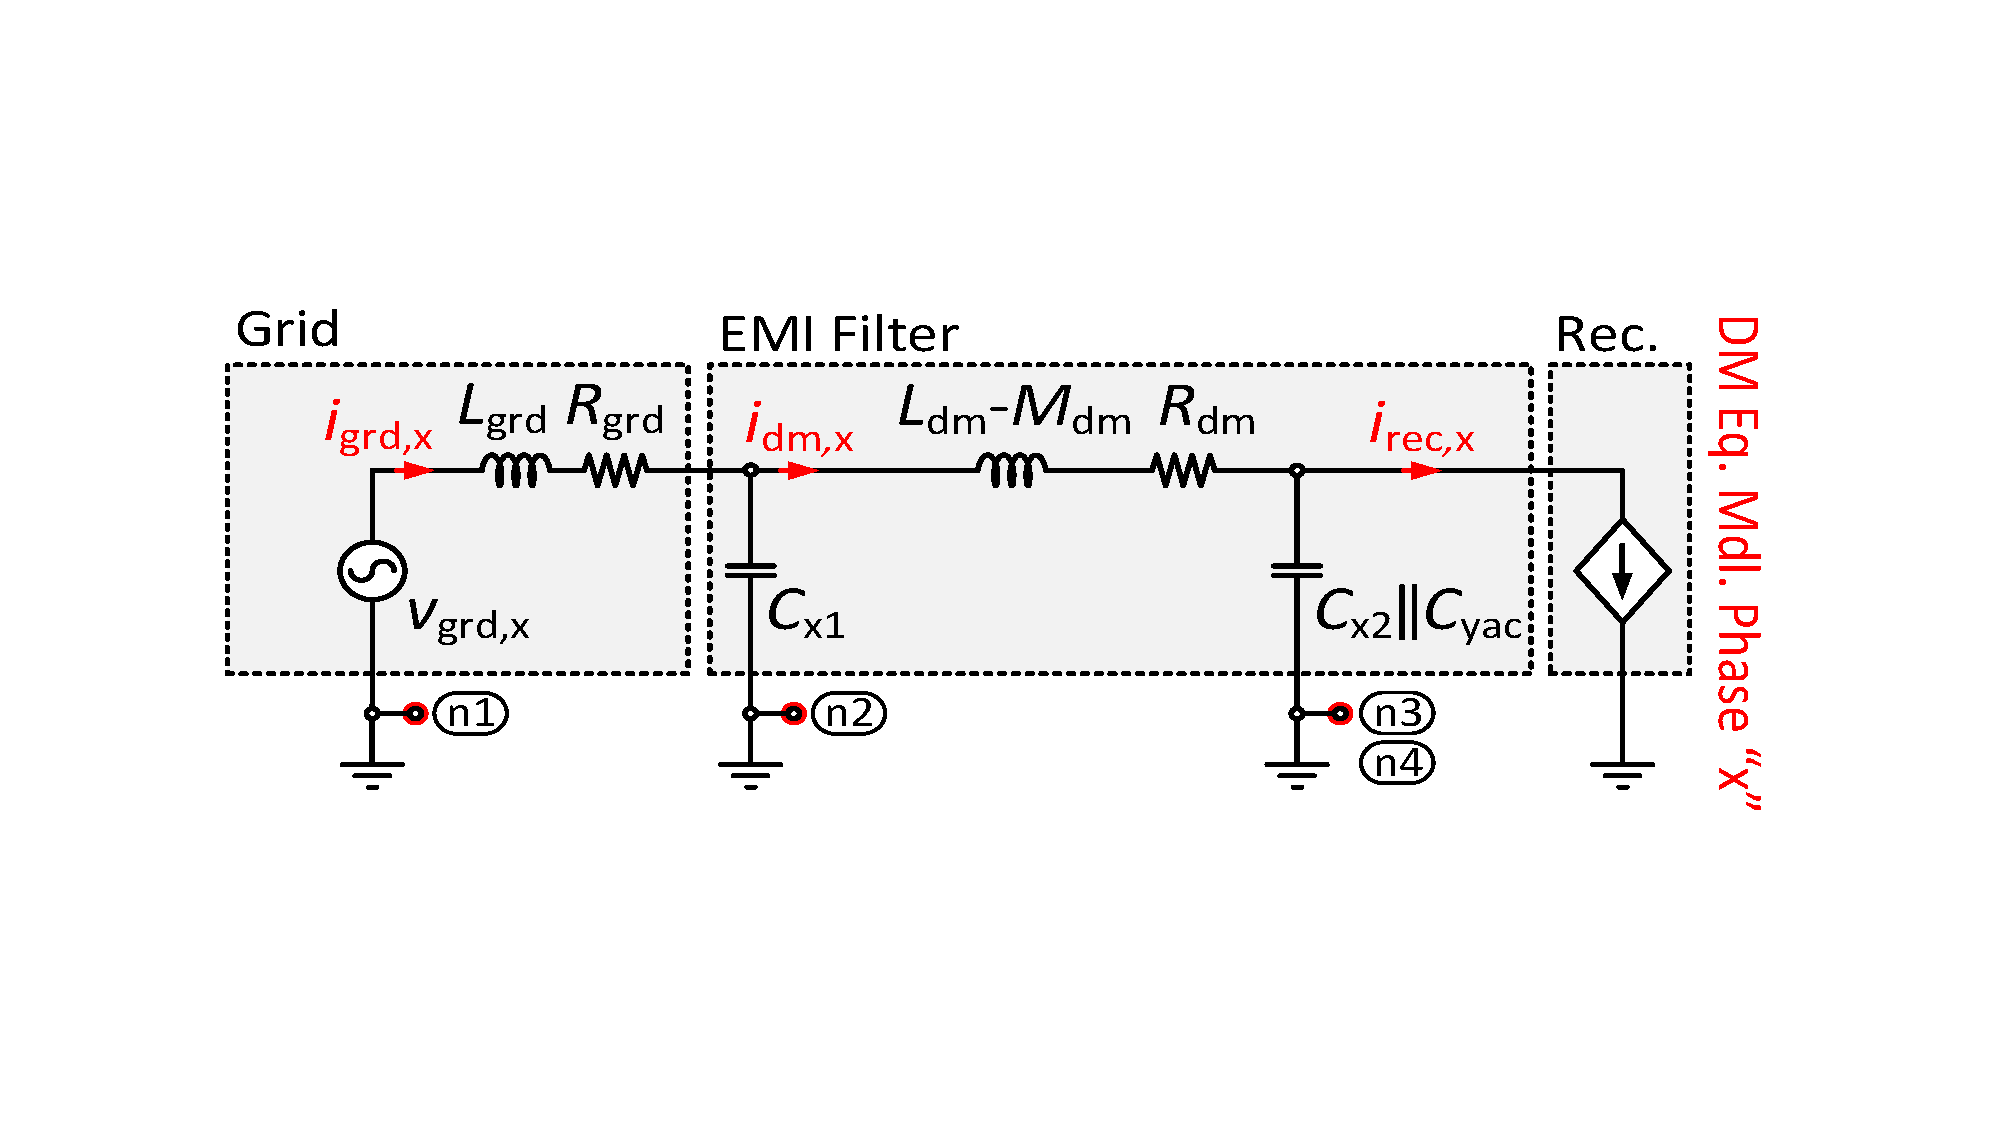
\includegraphics[clip, trim=0cm 5cm 0cm 4.5cm, width=1\linewidth]{FIGS/FIG_7B.pdf}
	                }
	    \end{center}
	    \vspace{-3mm}
	    \caption{Proposed equivalent model of the motor-drive system for (a) three-phase and (b) single-phase. {\color{red}\{I think the three-phase equivalent model is redundant.\}}}
	    \label{FIG7}
	\end{figure}
	
	%%FIG8
		\begin{figure*}[t]
			    \centering
			    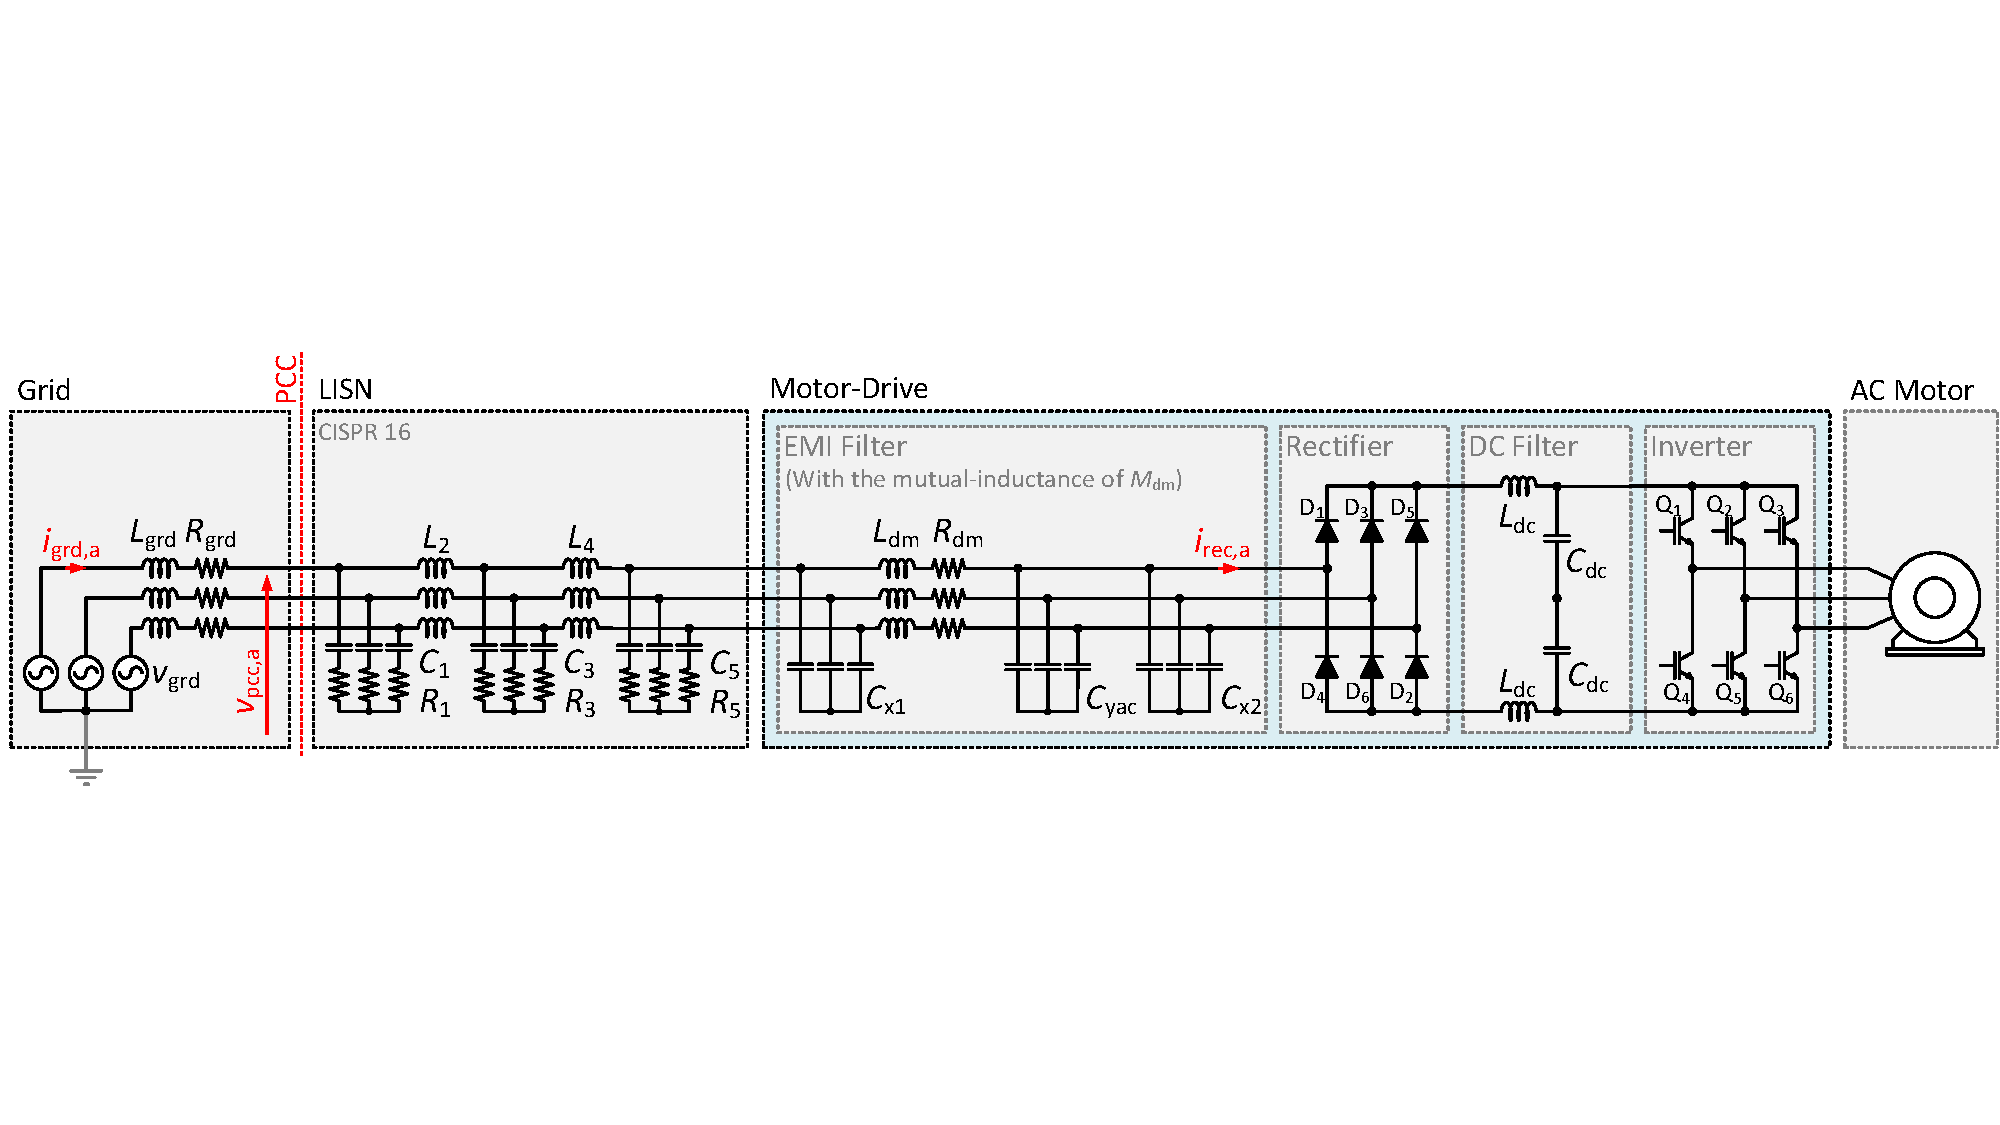
\includegraphics[clip, trim=0cm 5.5cm 0cm 5cm, width=1\linewidth]{FIGS/FIG_8.pdf}
			    \caption{The motor-drive system under study for common-mode EMI investigations equipped with LISN.}
			    \label{FIG8}
			    \vspace{-5mm}
	    \end{figure*}

	\section{Single-Phase Equivalent Model to Model DM EMI Caused by Three-Phase Rectifiers}
	This section explains some reasons for mode-changing transients. Then some approaches to model this phenomenon are discussed. Subsequently, the proposed technique for modeling the rectifier mode-changing transients is elaborated.
	
	To rectify the input three-phase currents ($i_{\mathrm{rec},x}$) to the output current ($i_\mathrm{rec}$), the rectifier changes its mode of operation every $60^\circ$ (according to the input three-phase voltage). In each mode, the flow of three-phase input currents is redirected to the output current. During each mode, only two diodes are ON, and the circulation of current is in two phases of the rectifier input terminals. Fig.~\ref{FIG3} shows one of these modes of operation, in which the rectifier output current is formed by the currents in phases ``a" and ``b". 
	
	{\color{blue} As the combination of load (AC motor), dc-choke, and dc-capacitance makes dominant poles at low frequencies, for the high-frequency DM noises, the network after the rectifier can be modeled as a current source, as shown in Figs.~\ref{FIG1} and \ref{FIG3}.}
	
	The commutation between two modes of operation in the rectifier causes a sudden change in the flow of current in the back-end grid and EMI-filter. As a result, depending on the characteristics of the grid and EMI filter impedances, the mode-changing transients can be transferred to the grid with different gains at different frequencies. As in each mode of operation, the input currents of the rectifier circulates between two phases, the resultant mode-changing transients are also carried through two phases. Hence, the resultant noises are categorized in DM type of EMI.
	
	To analyze the effect of grid and EMI filter impedances on the DM EMI noises generated by the rectifier, XX in [] proposed two-phase (2PH) approach. In this technique, the non-interactive phase of the motor-drive system is completely neglected from the analysis, and the network shown in Fig.~\ref{FIG3} is rearranged to what is shown in Fig.~\ref{FIG6}. The obtained transfer function linking $I_{\mathrm{rec,x}}$ to $I_{\mathrm{grd,x}}$ for this network can be obtained as given in \eqref{EQ6}.
	
	%%EQ6
	\begin{flalign}
	    H_\mathrm{2PH}=
	    \frac{I_\mathrm{grd,x}}{I_{\mathrm{rec,x}}}= &&\nonumber
	    \\
	    \frac{Z_{\mathrm{C,x1}}Z_{\mathrm{C,x2y}}}{Z_\mathrm{grd}Z_\mathrm{C,x1}+Z_\mathrm{dm}Z_\mathrm{grd}+Z_\mathrm{dm}Z_\mathrm{C,x1}+Z_\mathrm{C,x2y}Z_\mathrm{C,x1}+Z_\mathrm{C,x2y}Z_\mathrm{grd}}&&
	    \label{EQ6}
	\end{flalign}
	
	\noindent where, $Z_{\mathrm{C,x1}}=-\mathrm{j}/\left({C_{\mathrm{x1}}\omega}\right)$ is the impedance of $C_{\mathrm{x1}}$, $Z_{\mathrm{dm}}=R_\amthrm{dm}+\mathrm{j}\left(L_\mathrm{dm}-M_\mathrm{dm}\right)\omega$ is the single-phase equivalent impedance of the EMI coil, and $Z_{\mathrm{C,x2y}}=-\mathrm{j}/\left({C_{\mathrm{x2y}}\omega}\right)$ is the impedance of $C_{\mathrm{x2}}||C_{\mathrm{yac}}$.
	
	
	
	%an asymmetric combination between the grid voltage and rectifier. Therefore, the third non-interacting phase of the grid-EMI system (connected to the rectifier) makes an asymmetric coupling between the third phase of the grid to the grid currents. This situation is sequentially changed among different phases in each switching mode (every $60^\circ$) of the rectifier and (specially for a weakly damped system) makes it complex to relate the rectifier input currents ($i_{\mathrm{rec,x}}$) to the grid currents ($i_{\mathrm{grd,x}}$) and decouple the relationship from the grid voltages. 
	%{\color{red}\{XX in [] used three-phase conduction-mode model at the grid-side to map the input currents of the rectifier to the grid currents. In this approach, .... 
	{\color{red}Although this technique provides a simple approach to link the rectifier currents to the grid currents, it is not an accurate model due to neglecting the floated phase of the grid-EMI system.} {\color{red}\{This part stands for two-phase conduction-mode in Hansika's paper, and a reference is needed here for it.\}}
	
	Therefore, in this article, single-phase equivalent model is proposed as a trade-off between accuracy (proposed in []) and simplicity (discussed in []). In this approach, the three-phase system is considered to have decoupled phases, and each phase of the system is modelled to convert a phase of the rectifier input currents to a phase of the grid currents. This assumption is possible to be made owing to the zero net of current at KCL1, KCL2, and KCL3 in Fig.~\ref{FIG1} when the neutrals of the system are not connected to the ground. This means there is no common-mode current in the system. Hence, on the one hand, $v_\mathrm{n1}$, $v_\mathrm{n2}$, $v_\mathrm{n3}$, and $v_\mathrm{n4}$ are equal. On the other hand, the couplings of the EMI filter can be simplified into the self-inductances of the EMI inductors, and the coupled EMI inductors can be replaced by the decoupled self-inductance of $L_\mathrm{dm}-M_\mathrm{dm}$ in each phase. 
	
	Therefore, the three-phase system shown in Fig.~\ref{FIG1} can be simplified into what is shown in Fig.~\ref{FIG7}(a), in which the rectifier output currents are dispersed into three current sources $i_{\mathrm{rec,a}}$, $i_{\mathrm{rec,b}}$, and $i_{\mathrm{rec,c}}$ as explained in \eqref{EQ4} and \eqref{EQ5}. As the obtained three-phase system is decoupled from other two phases, it can be simplified into a single-phase (1PH) system as shown in Fig.~\ref{FIG7}(b). In this equivalent system, the transfer function that links $I_{\mathrm{rec},x}$ to $I_{\mathrm{grd},x}$ is as below.
	
	%%EQ7
	\begin{flalign}
	    H_\mathrm{EMI}=
	    \frac{I_\mathrm{grd,x}}{I_{\mathrm{rec,x}}}= &&\nonumber
	    \\
	    \frac{Z_{\mathrm{C,x1}}Z_{\mathrm{C,x2y}}}{Z_\mathrm{grd}Z_\mathrm{C,x1}+Z_\mathrm{dm}Z_\mathrm{grd}+Z_\mathrm{dm}Z_\mathrm{C,x1}+Z_\mathrm{C,x2y}Z_\mathrm{C,x1}+Z_\mathrm{C,x2y}Z_\mathrm{grd}}&&
	    \label{EQ7}
	\end{flalign}
	
	\noindent{\color{red} SAME EQUATION!!}
	
	{\color{red} \{Based on the analysis, there is no difference between the two-phase model and the single-phase model.\}}  
	
    %%FIG9
	\begin{figure}[t]
	    \begin{center}
	        \subfloat[]{
	                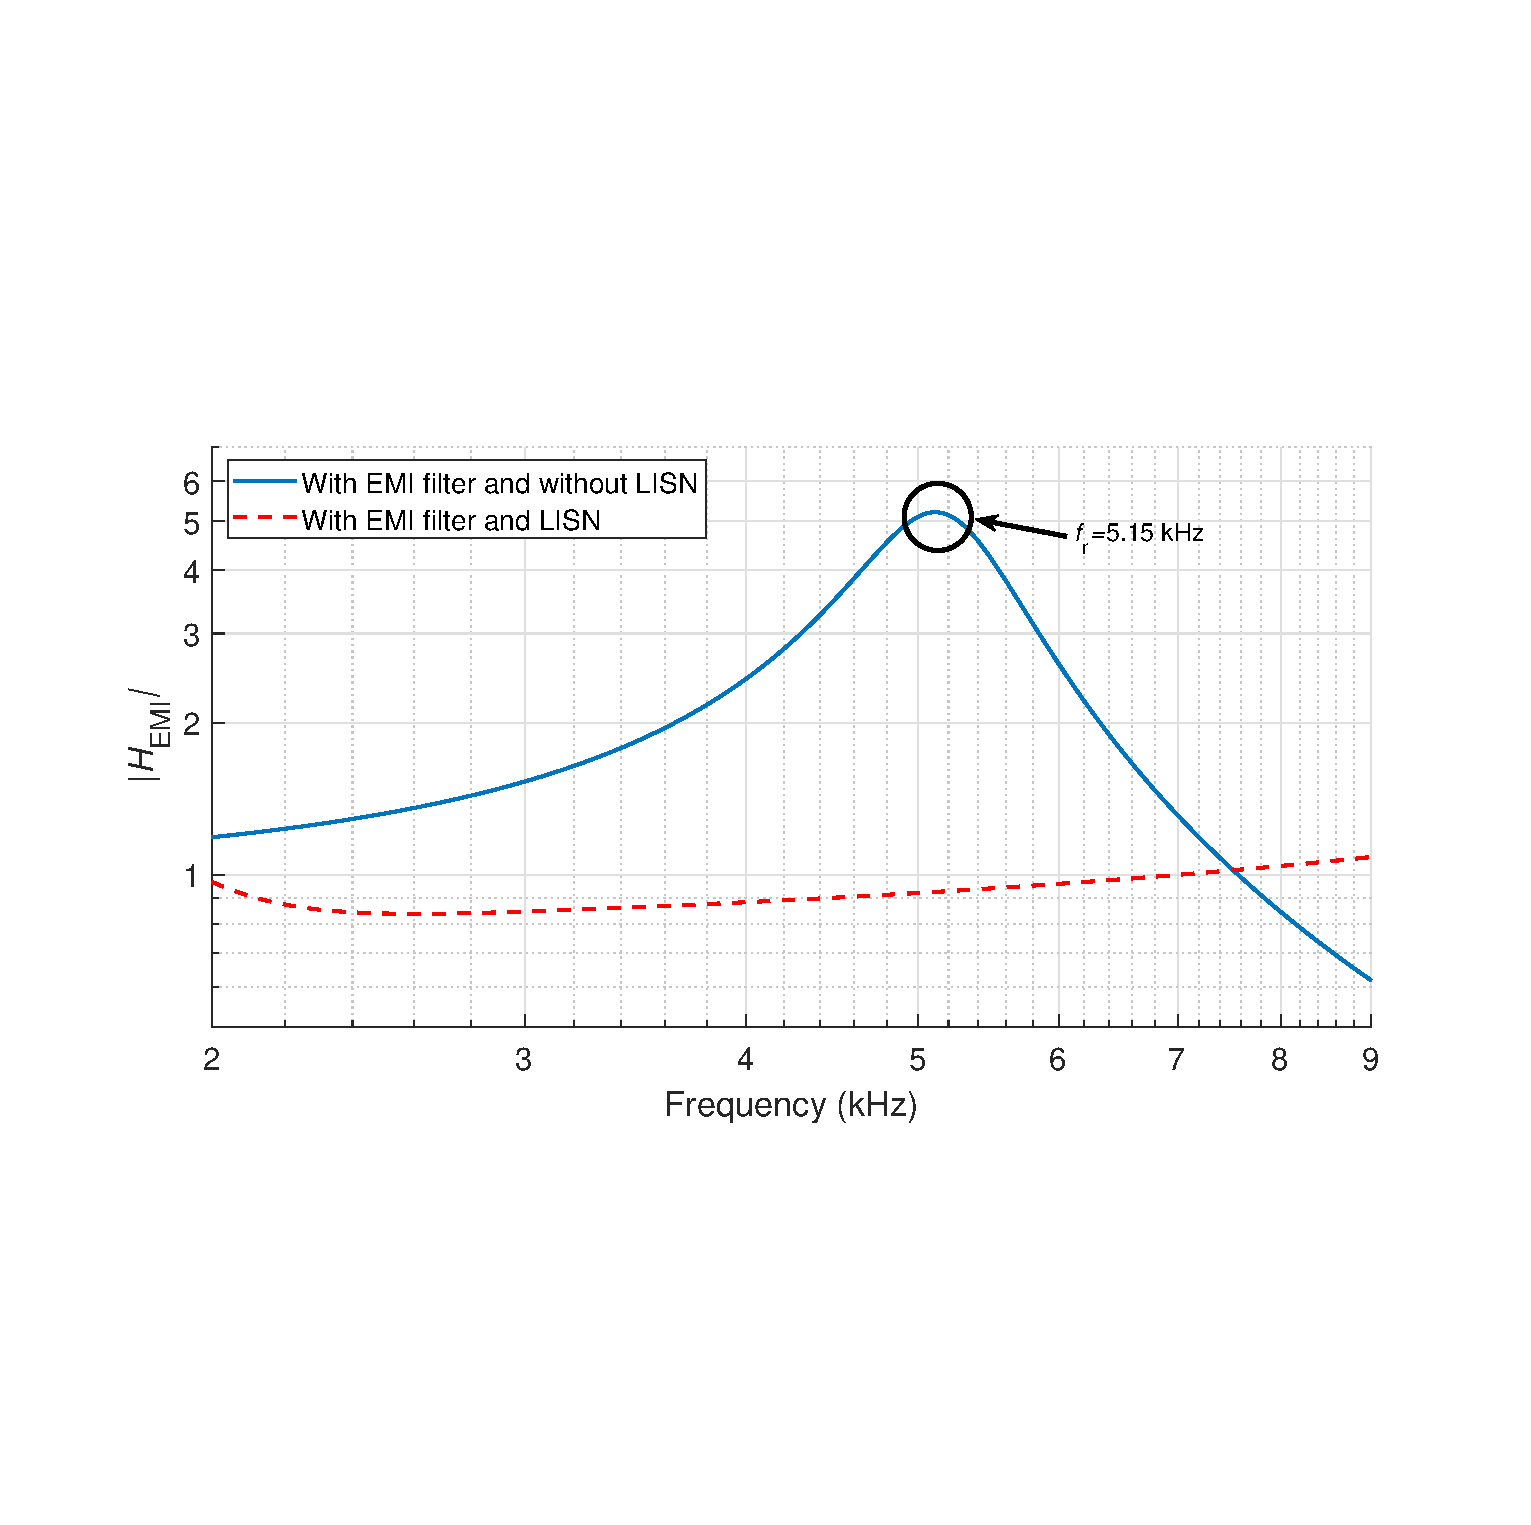
\includegraphics[clip, trim=1.25cm 6.5cm 1.25cm 7cm, width=1\linewidth]{FIGS/FIG_9A.eps}
	                }
	                \\
	                \vspace{-3mm}
	        \subfloat[]{
	                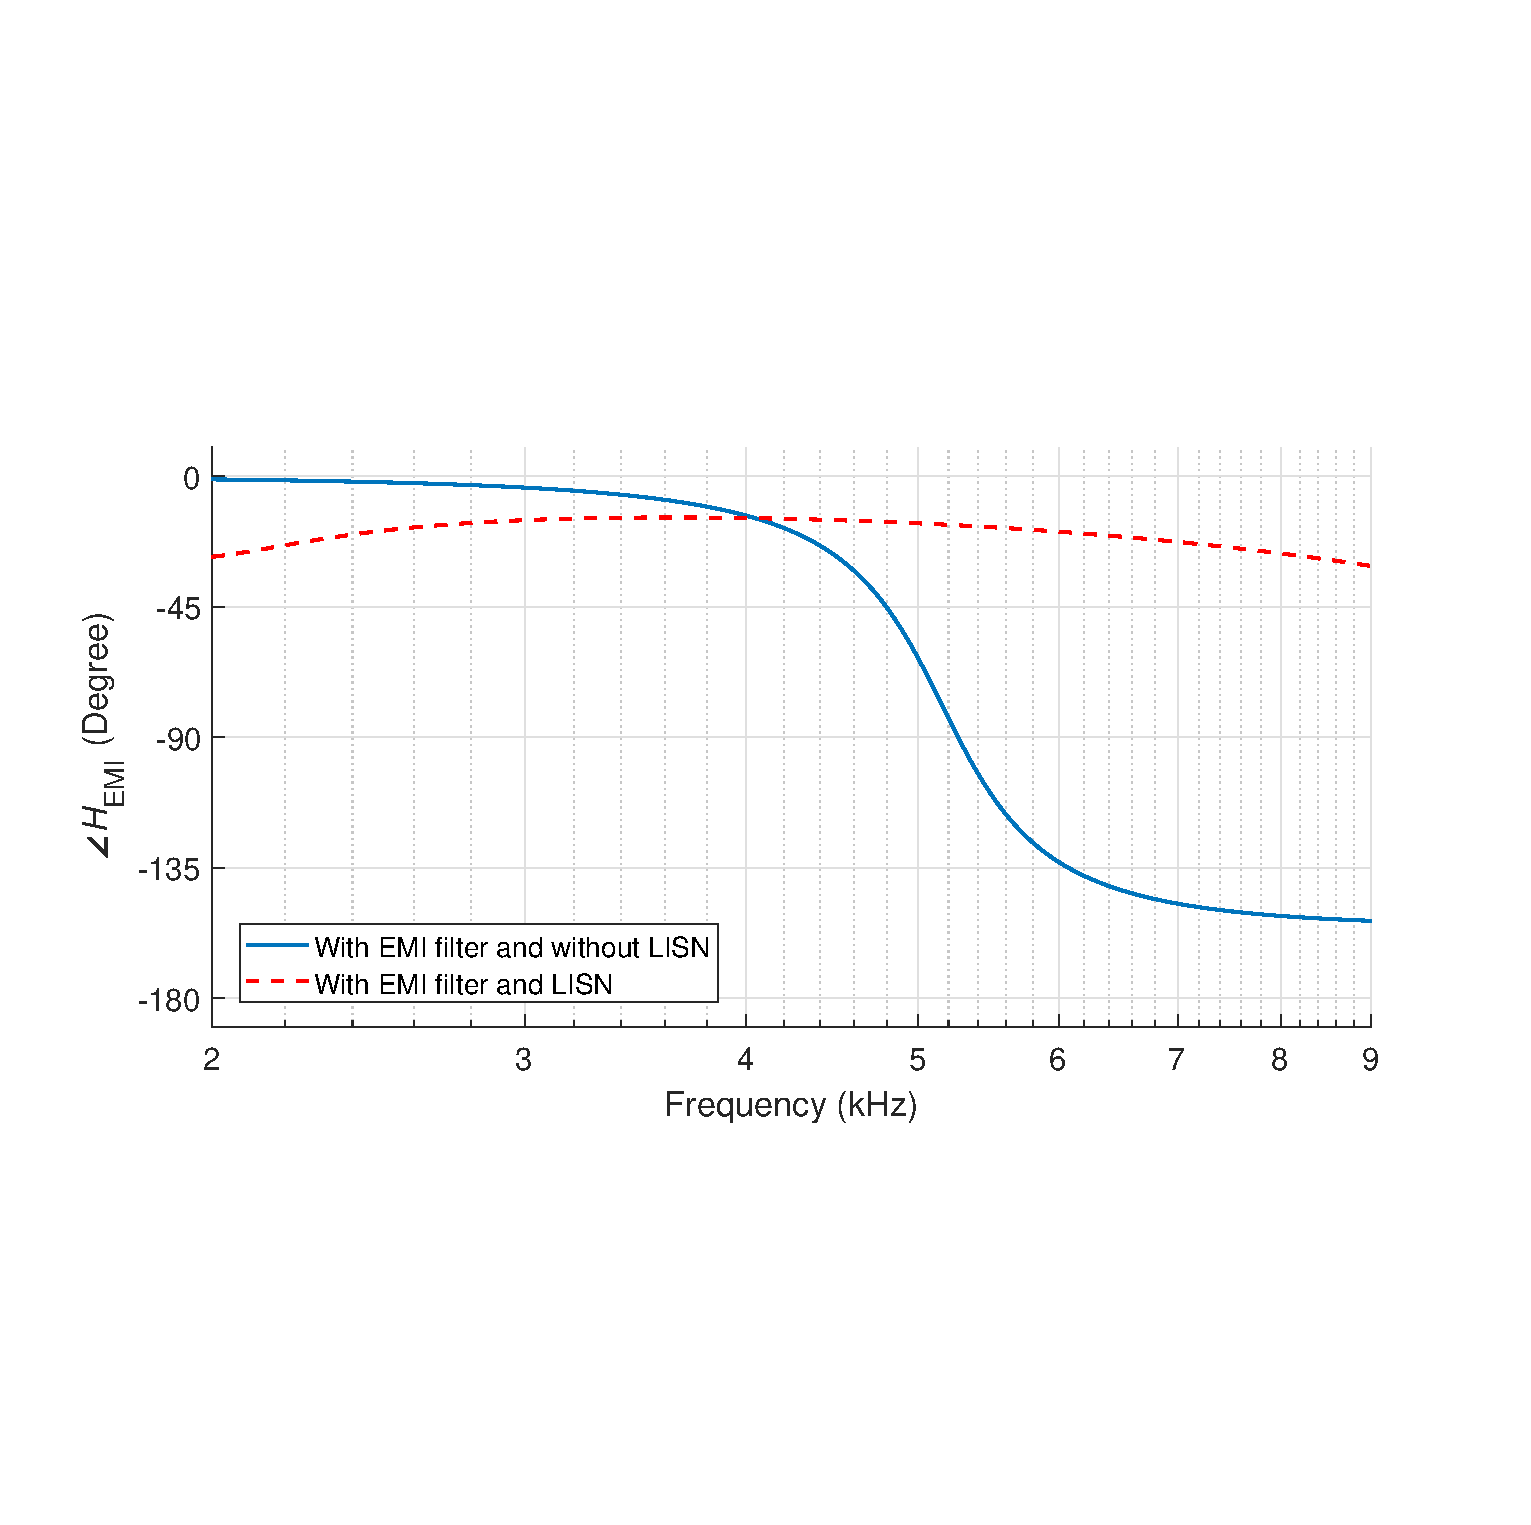
\includegraphics[clip, trim=1.25cm 6.5cm 1.25cm 7cm, width=1\linewidth]{FIGS/FIG_9B.eps}
	                }
	    \end{center}
	    \vspace{-3mm}
		\caption{Bode diagram of $H_\mathrm{EMI}$ when the motor-drive setup is equipped only with EMI filter (solid blue line) and when it is equipped with both EMI filter and LISN (red dashed line). (a) amplitude of the EMI transfer function ($|\textit{H}_{\textrm{EMI}}|$) and (b) angle of the EMI transfer function ($\angle \textit{H}_{\textrm{EMI}}$).}
		\label{FIG9}
	\end{figure}
	
	%%FIG10
	\begin{figure}
	    \begin{center}
	       % \subfloat[]{
	       %         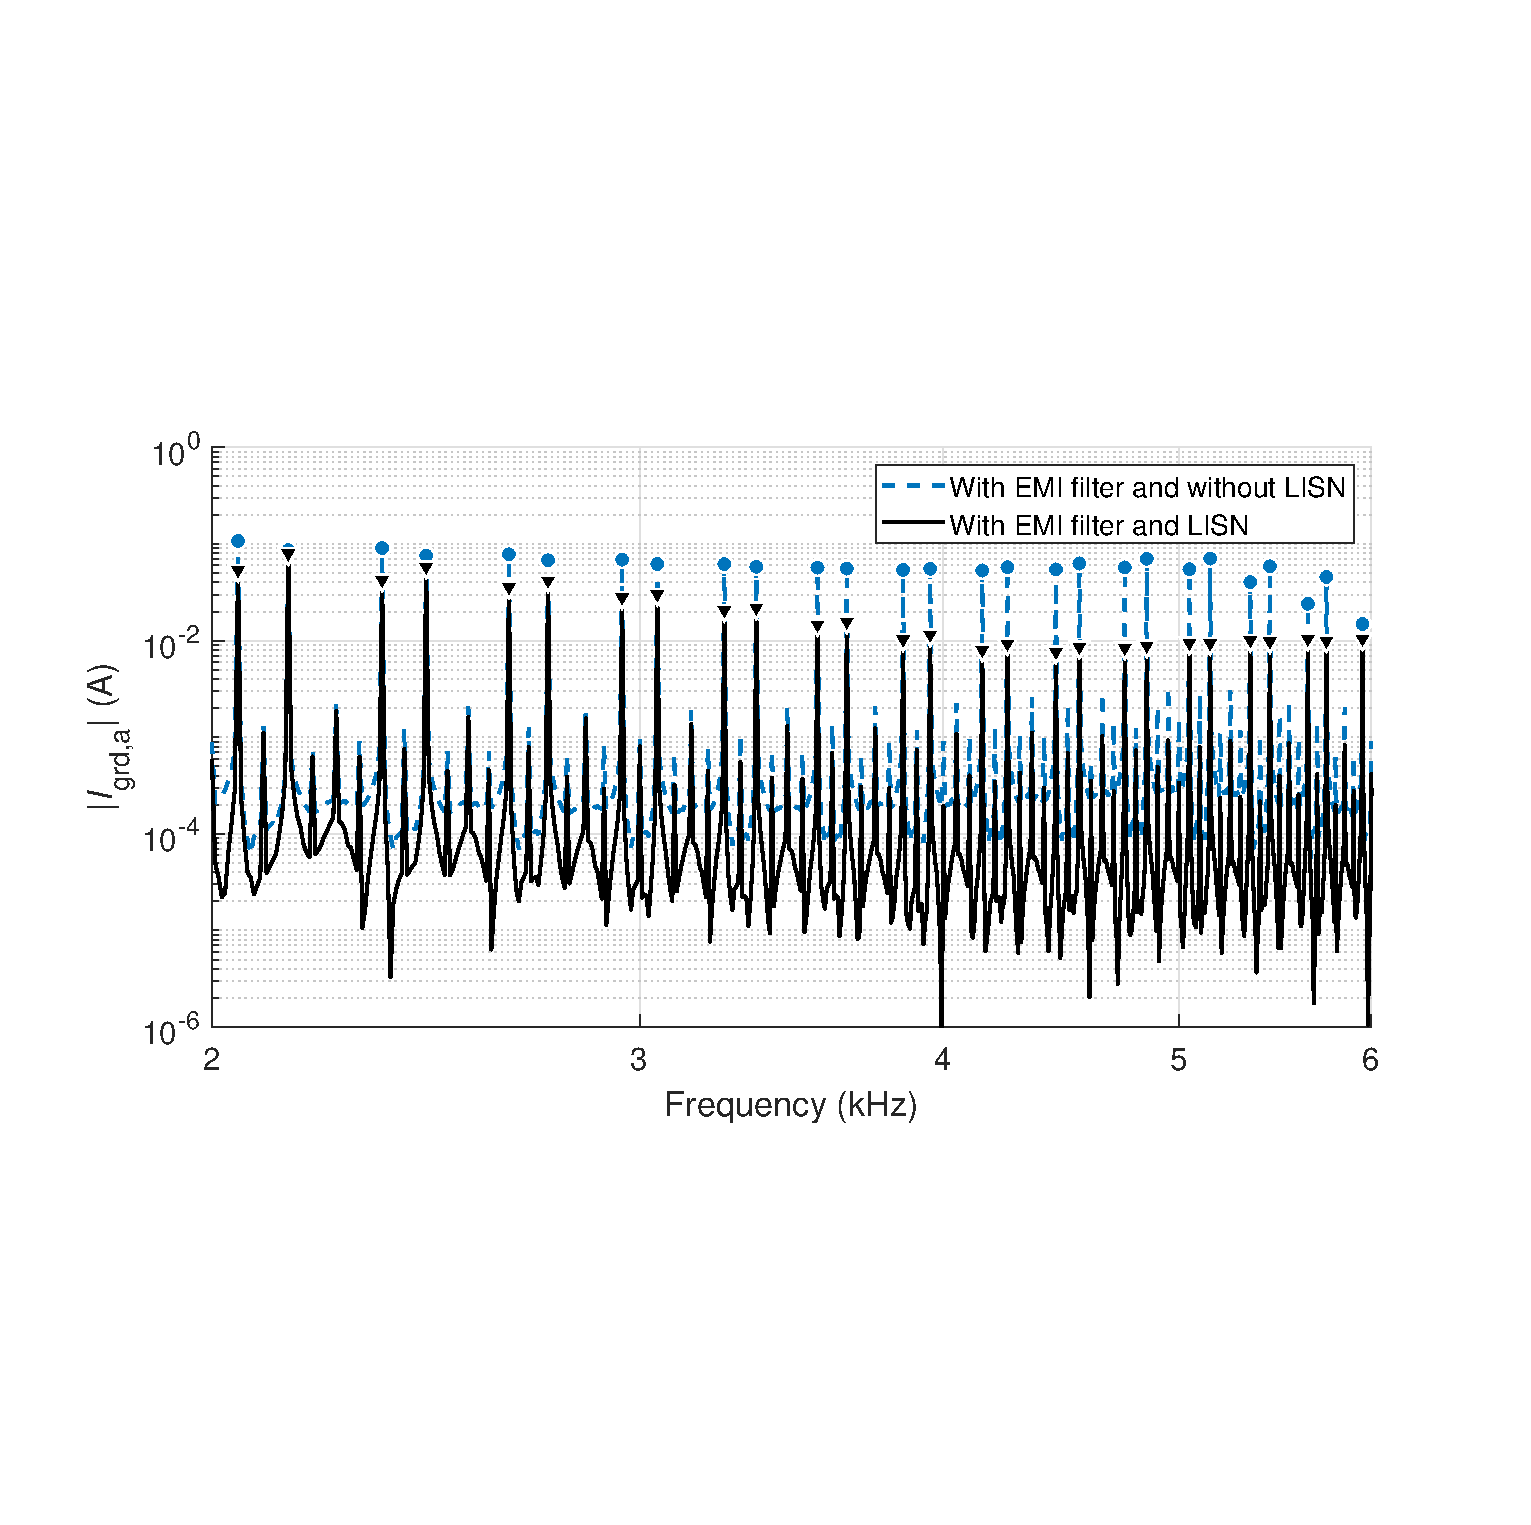
\includegraphics[clip, trim=1.25cm 6.5cm 1.25cm 7cm, width=1\linewidth]{FIGS/FIG_11A.eps}
	       %         }
	       %         \\
	       %         \vspace{-3mm}
	       % \subfloat[]{
	                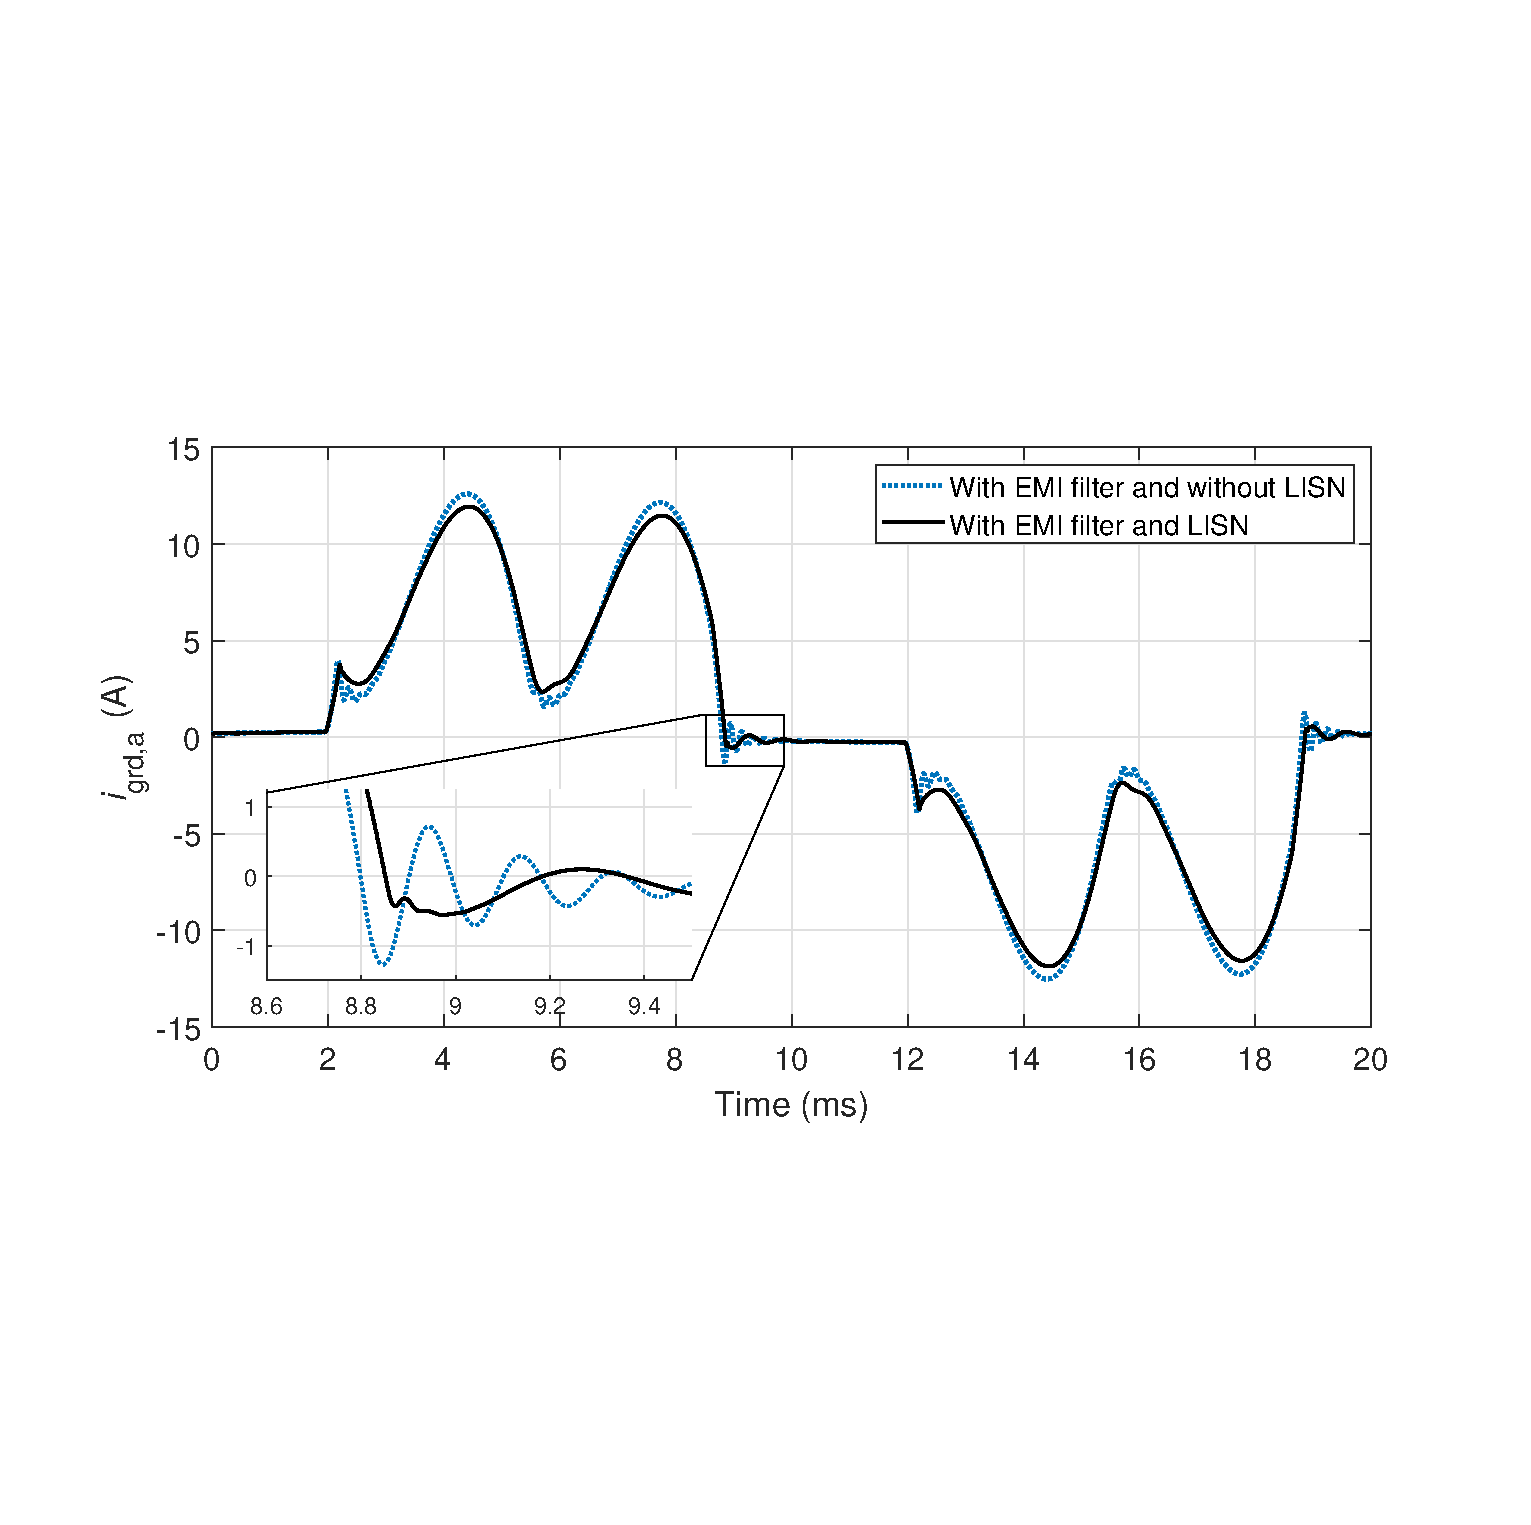
\includegraphics[clip, trim=1.25cm 6.5cm 1.25cm 7cm, width=1\linewidth]{FIGS/FIG_10.eps}
	               % }
	    \end{center}
	    \vspace{-3mm}
	    %\caption{Time-domain results for (a) the PCC voltage $v_{\mathrm{pcc,a}}$ and (b) grid current $i_{\mathrm{grd,a}}$ when the system is not equipped with EMI filter and LISN (red dashed line), when the system is only equipped with EMI filter (blue dotted line), and when the system has both EMI filter and LISN (solid black line)}
	    \caption{Time-domain results for the grid current $i_{\mathrm{grd,a}}$ when the system is only equipped with EMI filter (blue dotted line) and when the system has both EMI filter and LISN (solid black line)}
	    \label{FIG11}
	\end{figure}
	
	%% FIG11
	\begin{figure}[t]
	    \centering
	    \subfloat[]{
		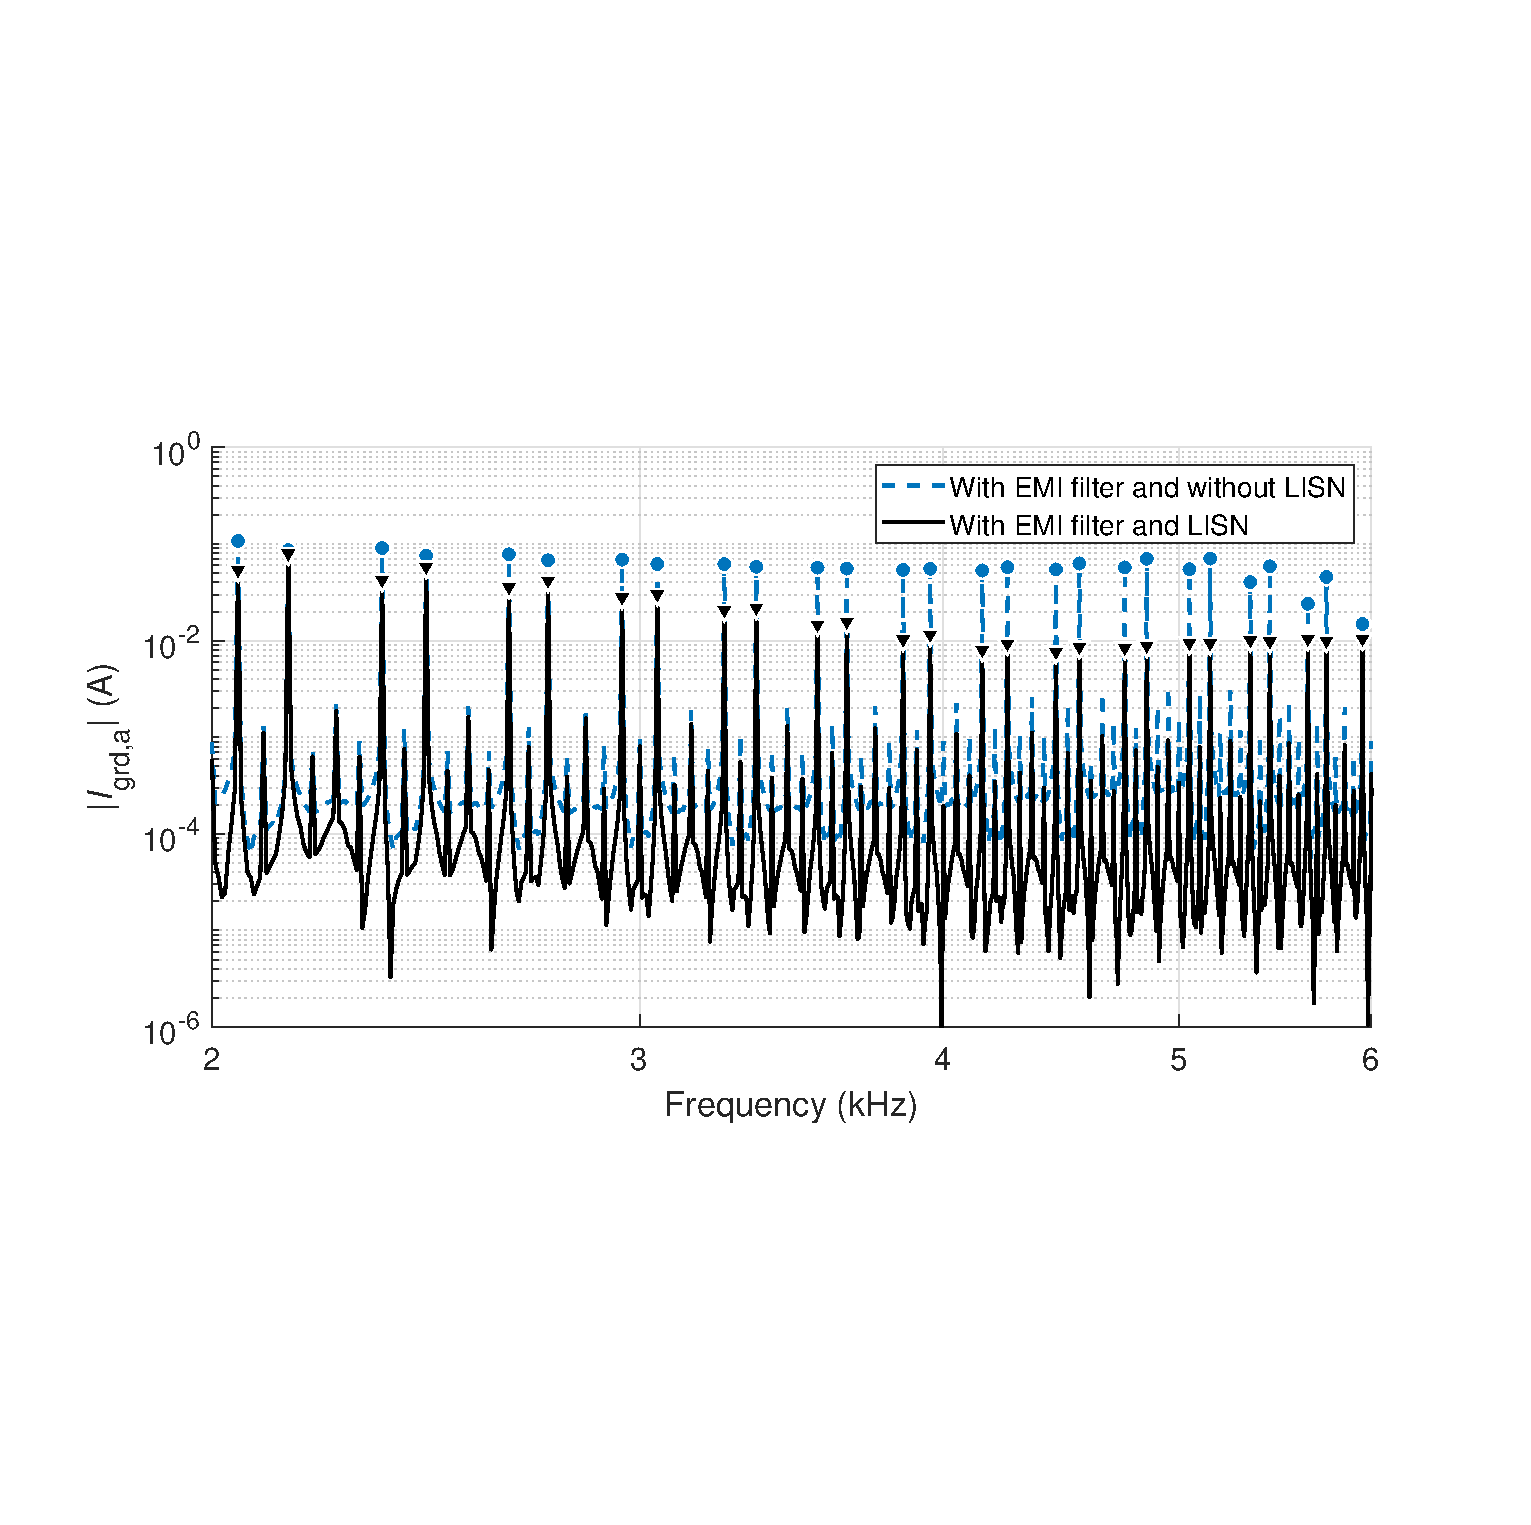
\includegraphics[clip, trim=1.25cm 6.5cm 1.25cm 7cm, width=1\linewidth]{FIGS/FIG_11A.eps}
		}\\
		\vspace{-3mm}
		\subfloat[]{
		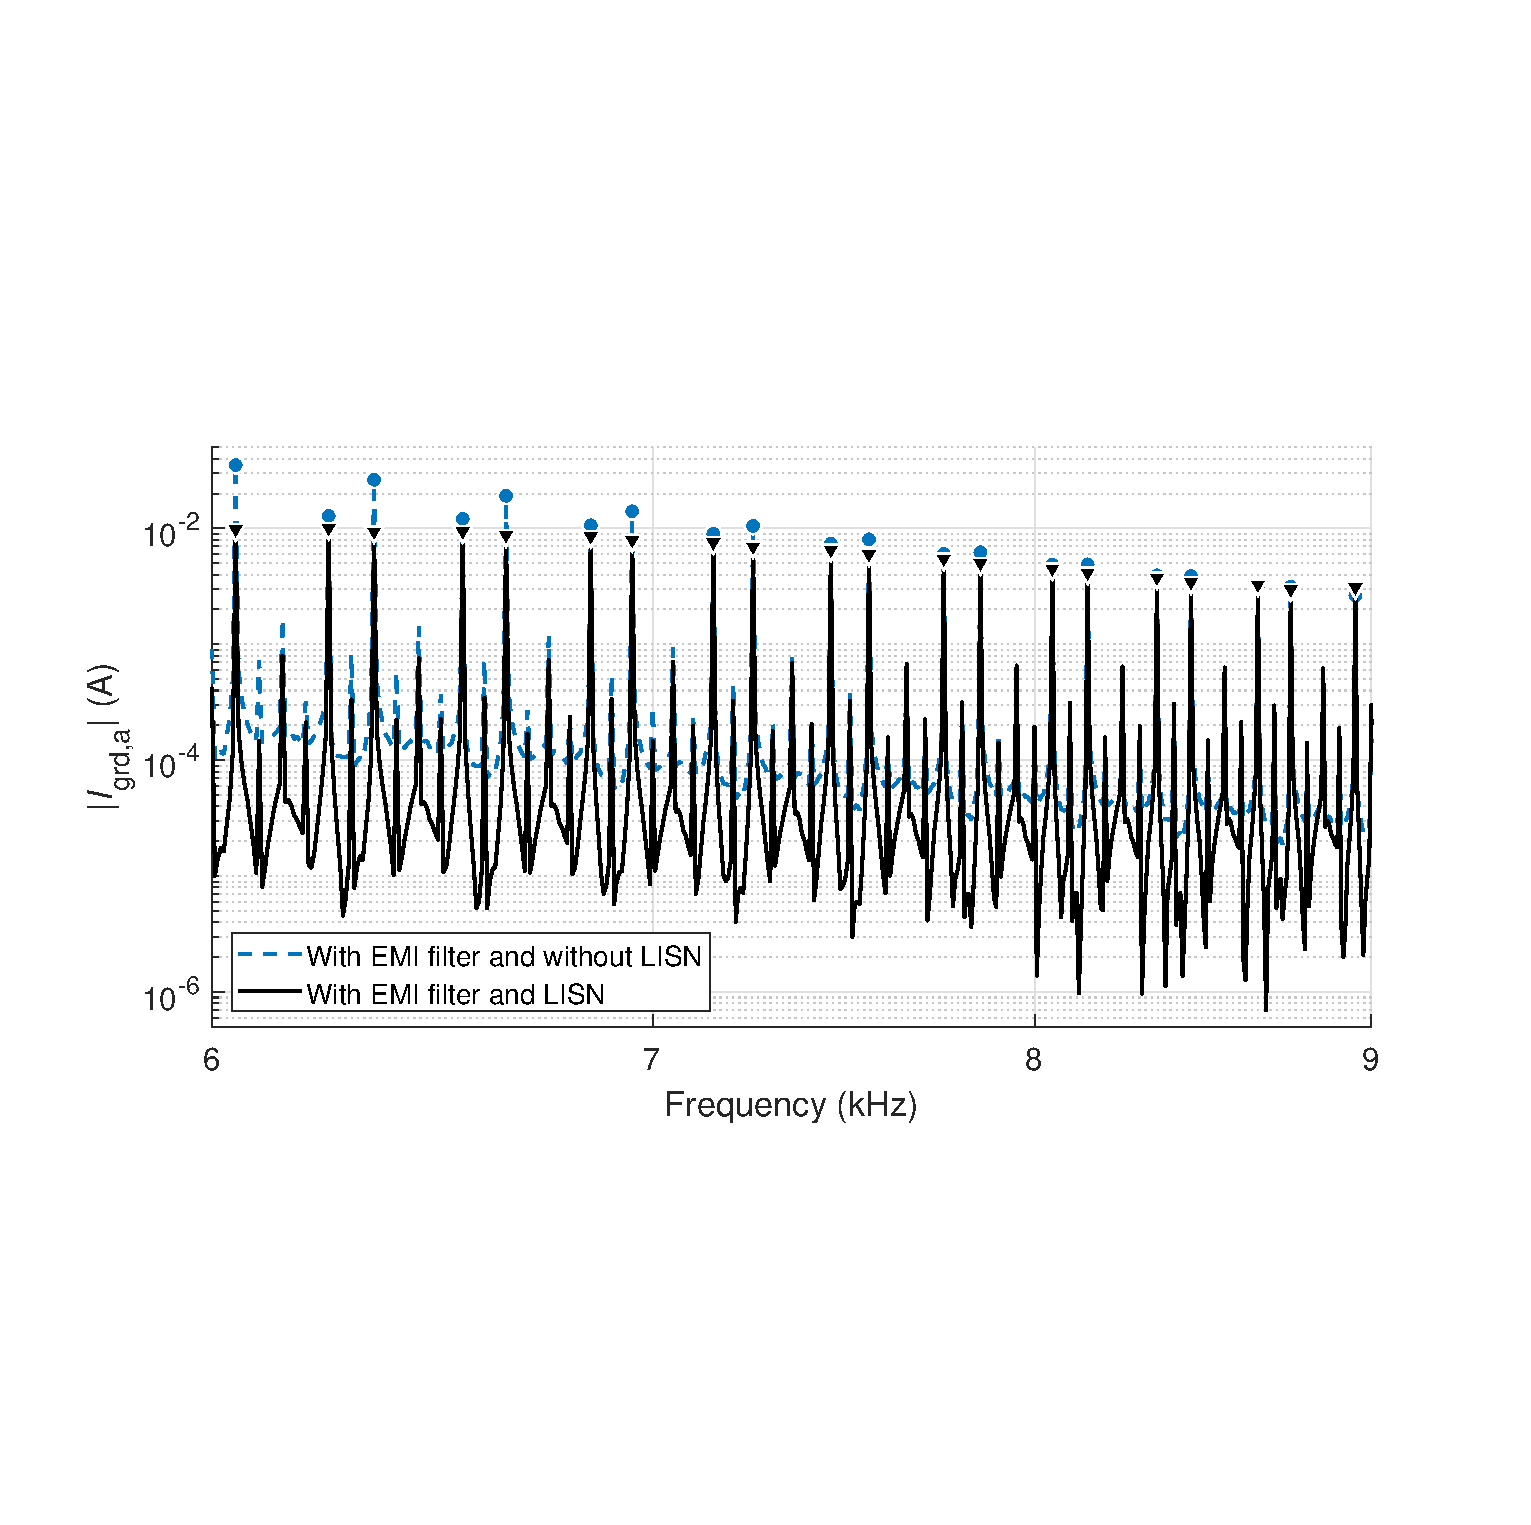
\includegraphics[clip, trim=1.25cm 6.5cm 1.25cm 7cm, width=1\linewidth]{FIGS/FIG_11B.eps}
		}
		\caption{Frequency-domain results for the grid current $|I_{\mathrm{pcc,a}}|$ and when the system is not equipped with EMI filter and LISN (red dashed line with rectangular red markers), when the system is only equipped with EMI filter (blue dotted line with circular blue markers), and when the system has both EMI filter and LISN (solid black line with triangular black markers) for the frequency ranges of (a) 2-6 kHz and (b) 6-9 kHz.}
		\label{FIG11}
	\end{figure}
    
    %%FIG12
	\begin{figure}
	    \begin{center}
	       % \subfloat[]{
	       %         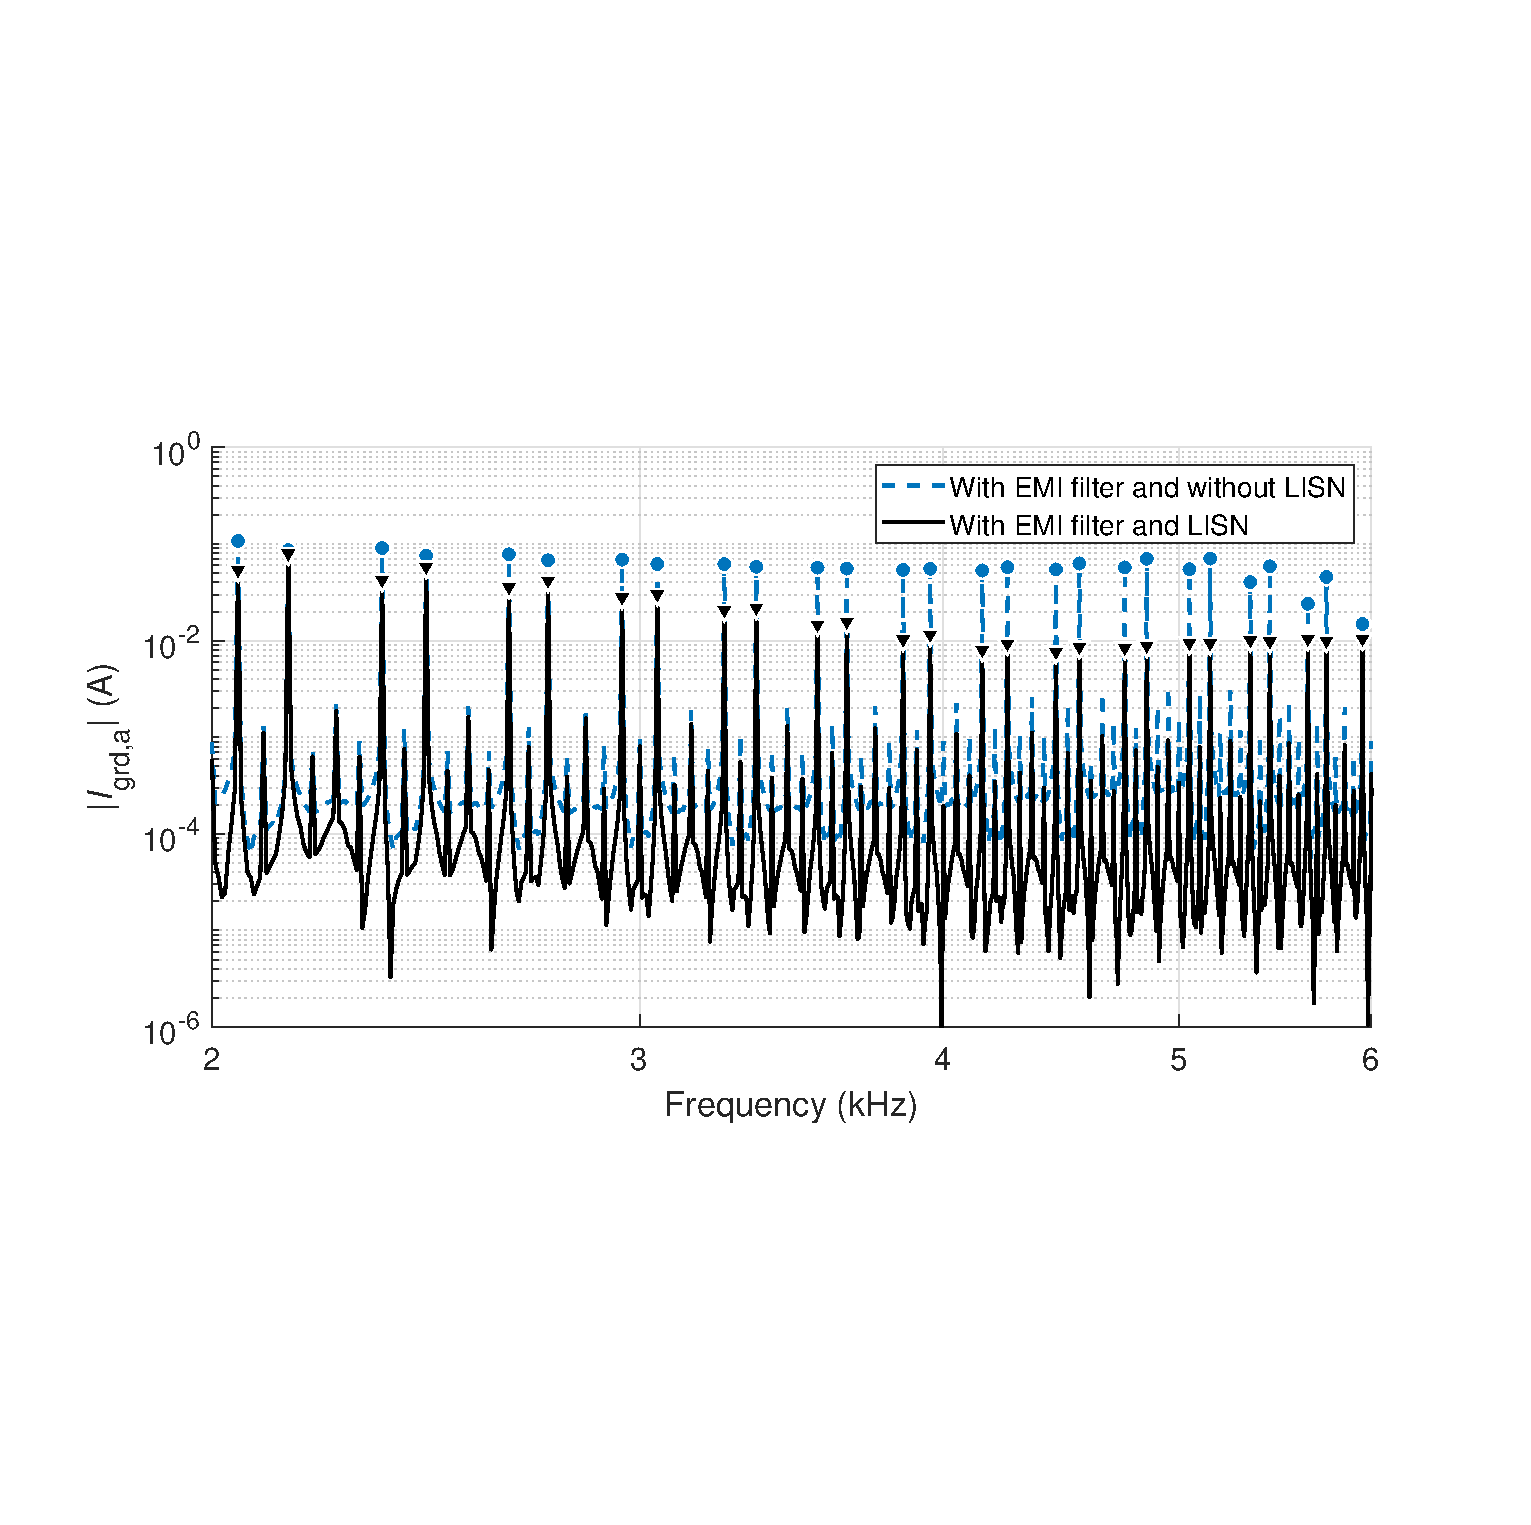
\includegraphics[clip, trim=1.25cm 6.5cm 1.25cm 7cm, width=1\linewidth]{FIGS/FIG_11A.eps}
	       %         }
	       %         \\
	       %         \vspace{-3mm}
	       % \subfloat[]{
	                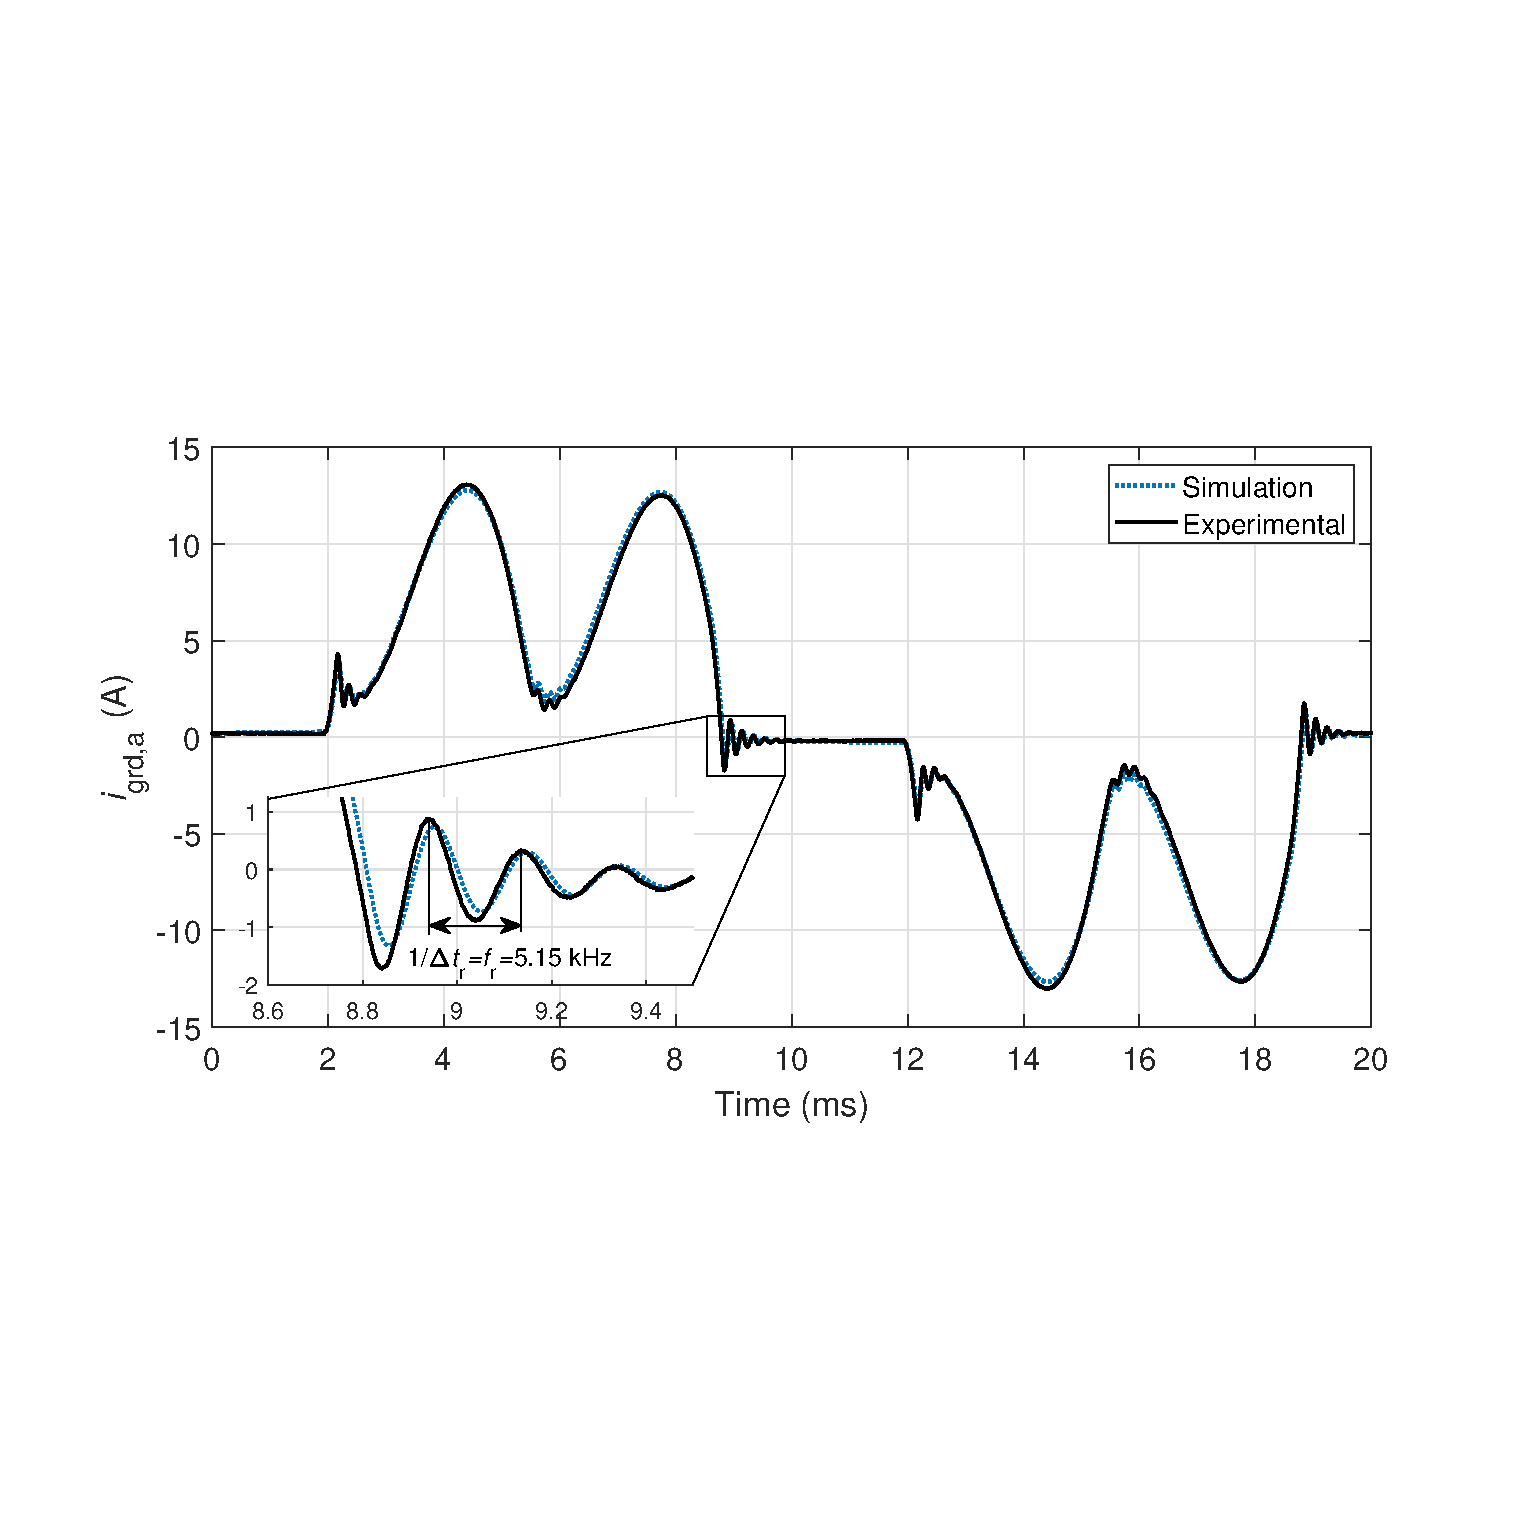
\includegraphics[clip, trim=1.25cm 6.5cm 1.25cm 7cm, width=1\linewidth]{FIGS/FIG_12.eps}
	               % }
	    \end{center}
	    \vspace{-3mm}
	    %\caption{Time-domain results for (a) the PCC voltage $v_{\mathrm{pcc,a}}$ and (b) grid current $i_{\mathrm{grd,a}}$ when the system is not equipped with EMI filter and LISN (red dashed line), when the system is only equipped with EMI filter (blue dotted line), and when the system has both EMI filter and LISN (solid black line)}
	    \caption{Time-domain simulation and experimental results for the grid current $i_{\mathrm{grd,a}}$ when the system is only equipped with EMI filter.}
	    \label{FIG11}
	\end{figure}
	
	%% FIG13
	\begin{figure}[t]
	    \centering
	    \subfloat[]{
		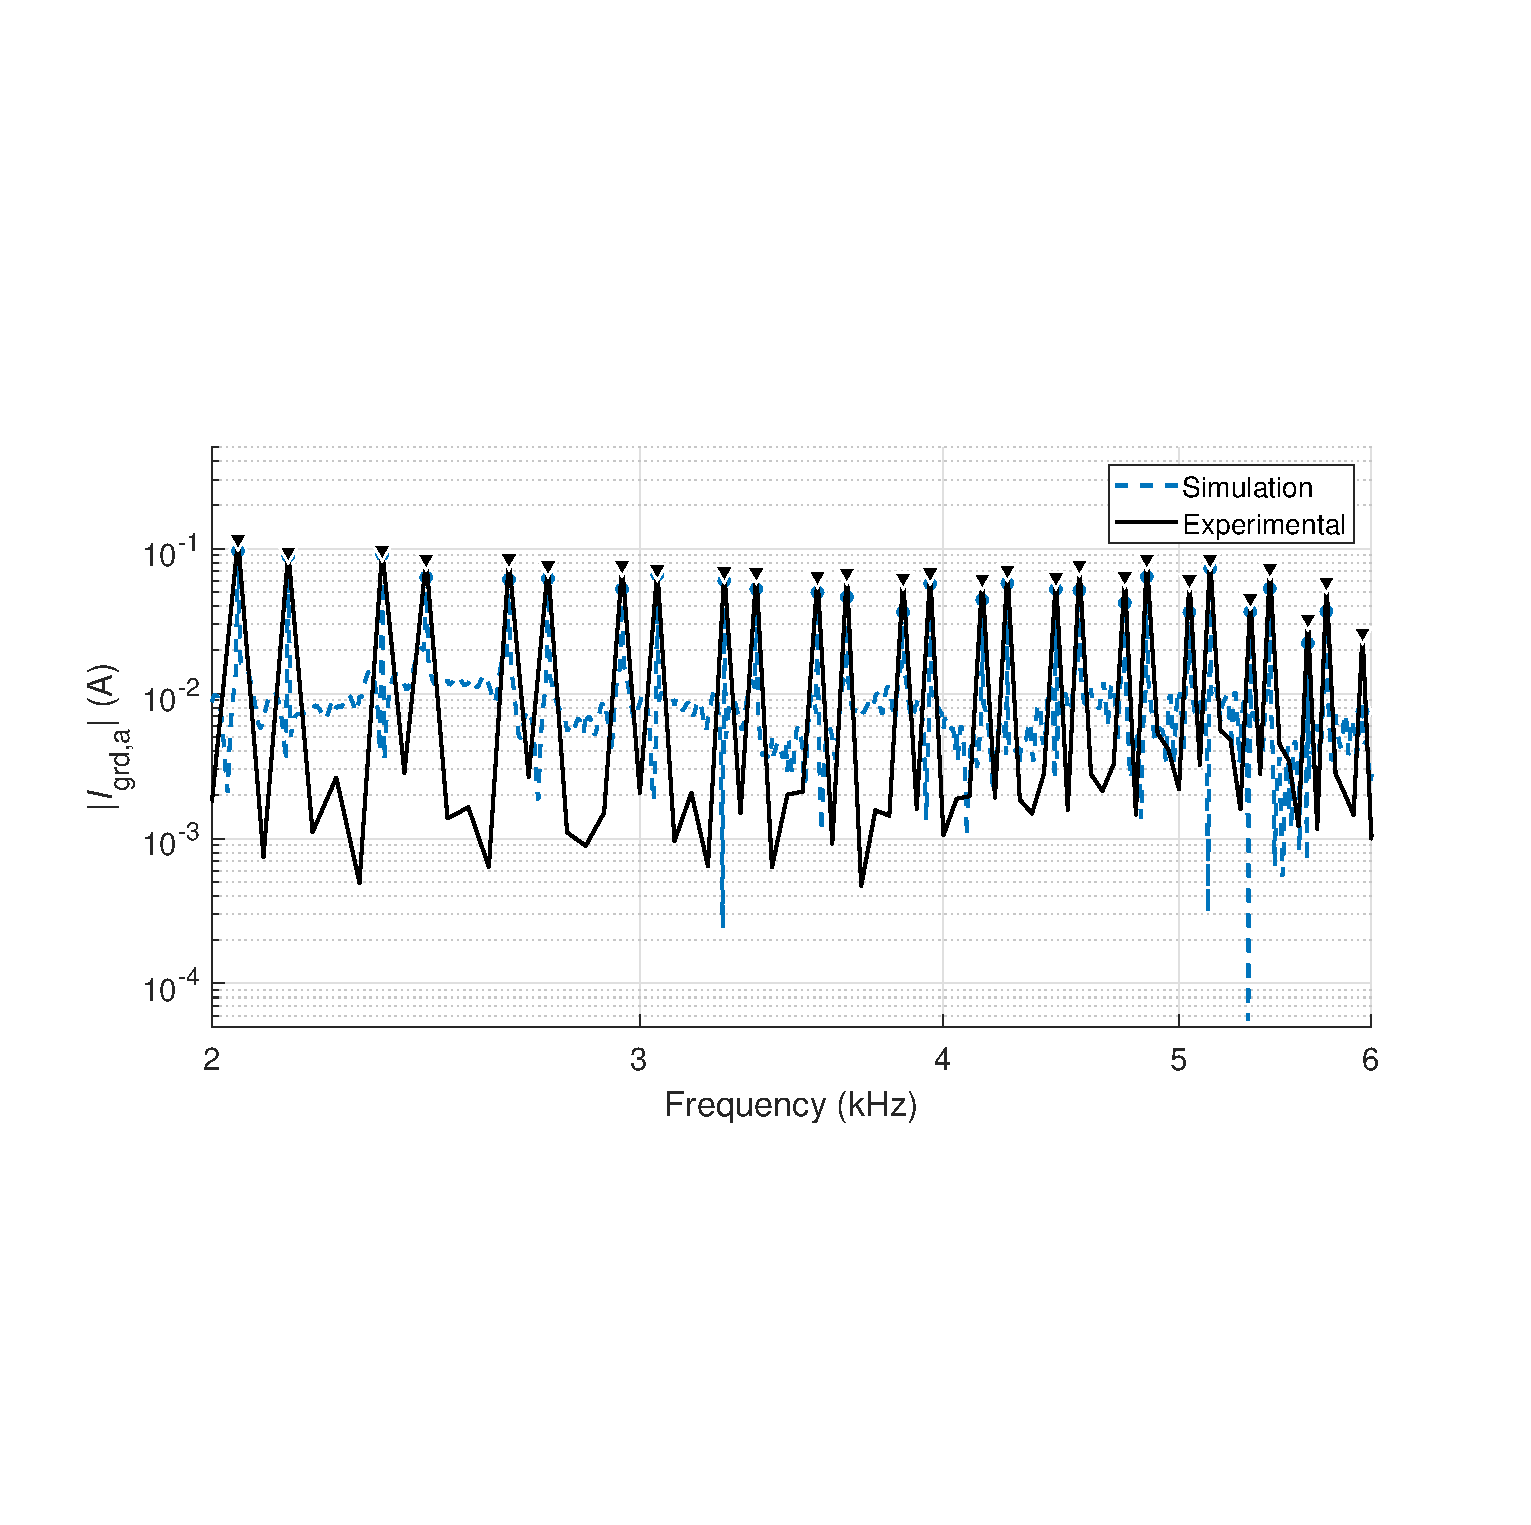
\includegraphics[clip, trim=1.25cm 6.5cm 1.25cm 7cm, width=1\linewidth]{FIGS/FIG_13A.eps}
		}\\
		\vspace{-3mm}
		\subfloat[]{
		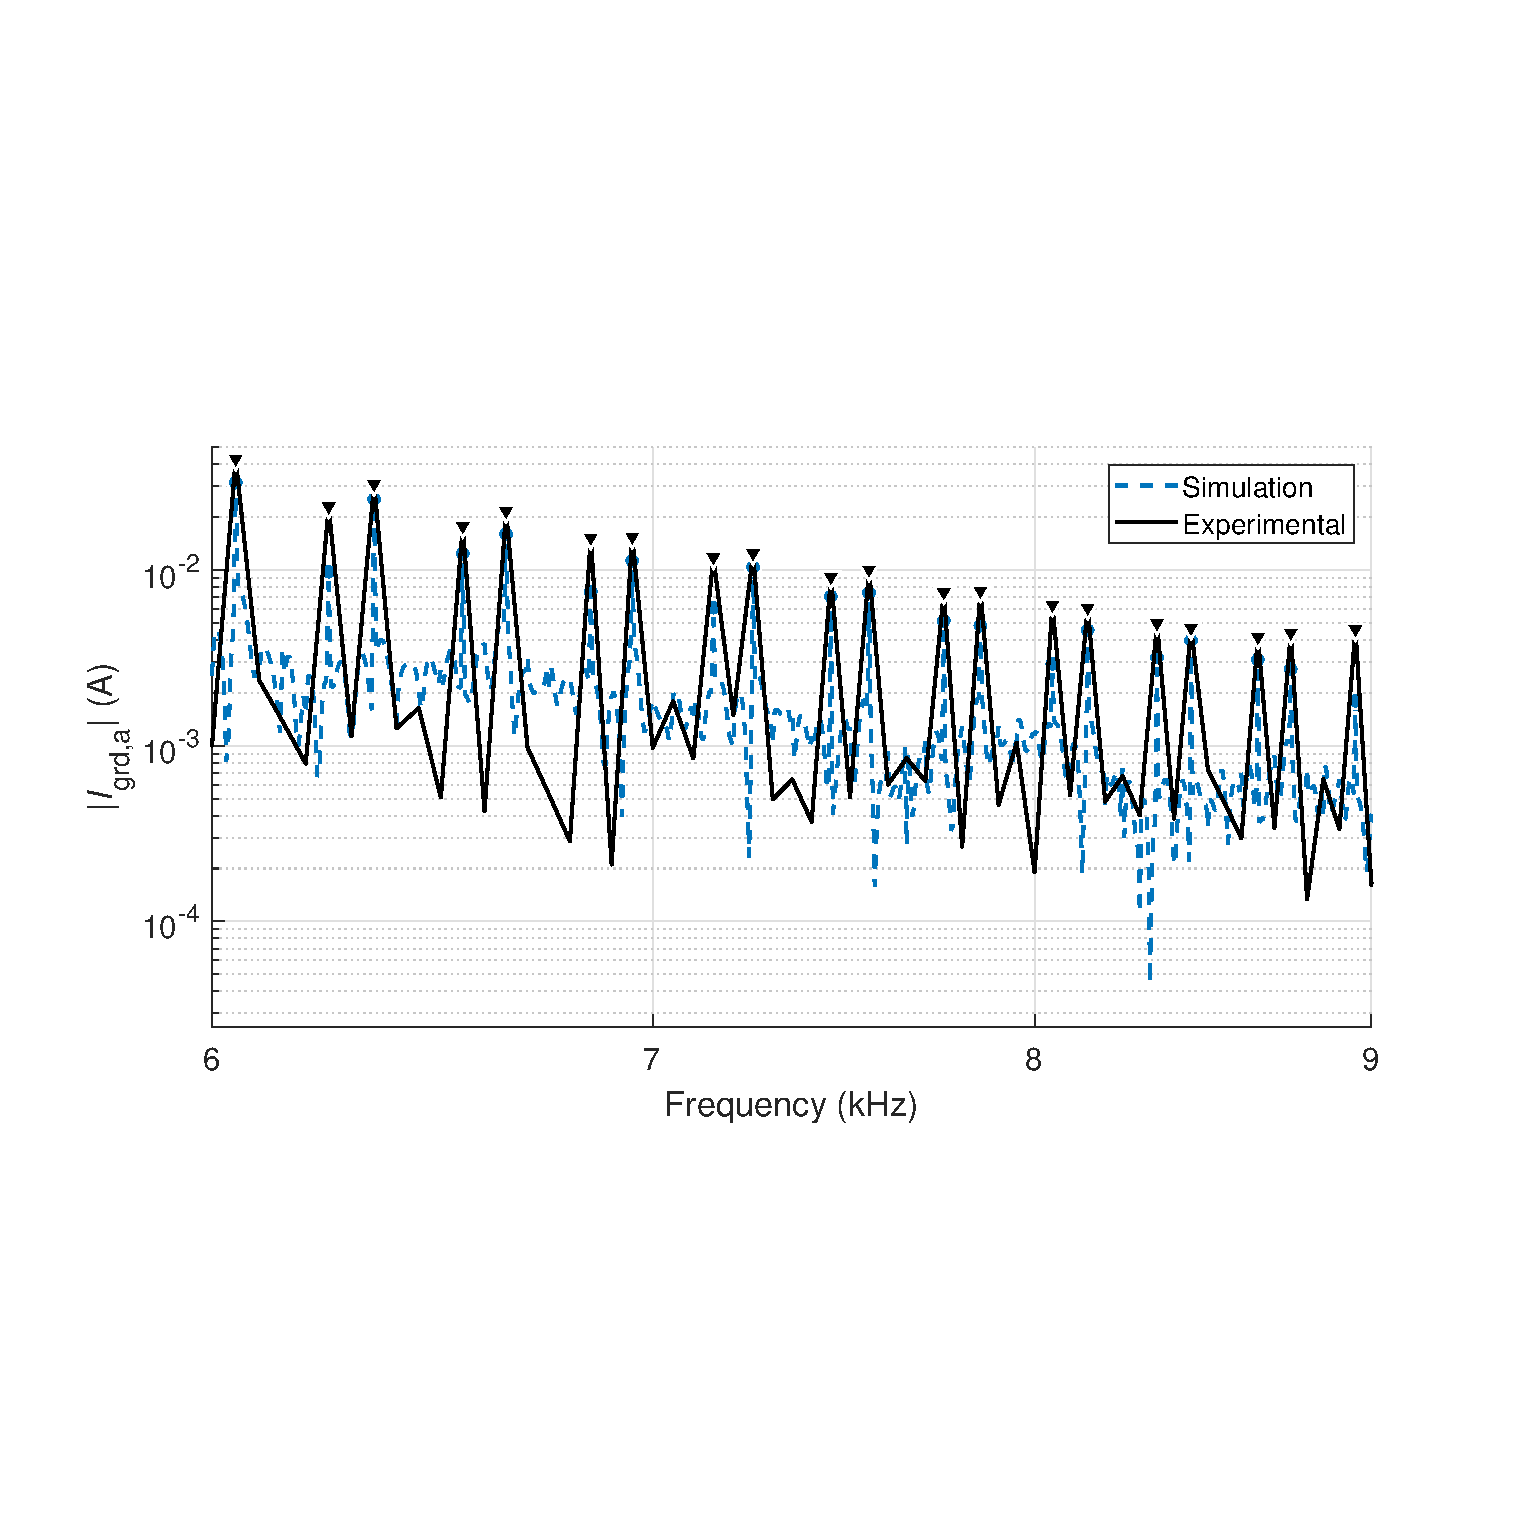
\includegraphics[clip, trim=1.25cm 6.5cm 1.25cm 7cm, width=1\linewidth]{FIGS/FIG_13B.eps}
		}
		\caption{Frequency-domain simulation and experimental results for the grid current $|I_{\mathrm{grd,a}}|$ and when the system is only equipped with EMI filter for the frequency ranges of (a) 2-6 kHz and (b) 6-9 kHz.}
		\label{FIG11}
	\end{figure}
    
    To investigate the effect of EMI filter on the propagation of DM EMI into the grid-side, the motor-drive system with and without line impedance stabilization network (LISN) is studied, and for each case, the effect of grid resistance $R_{\mathrm{grd}}$ on the mode changing transients is considered. Following, each case (with and without LISN) with different values of $R_\rm{grd}$ is investigated.
    
    \subsubsection{Motor-Drive System Without LISN}
    In the first test scenario, system shown in Fig.~\ref{FIG1} is considered which is not equipped with the LISN. This system resembles a realistic motor-drive system. The Bode diagrams of the motor-drive system without LISN and with grid resistances of $R_\mathrm{grd}=0.1~\Omega$ and $R_\mathrm{grd}=1~\Omega$ are shown in Fig.~\ref{FIG9}. As it is clear in this diagram, the $H_\mathrm{EMI}$ increases extensively around its resonant frequency, {\color{red} which is 5.15 kHz}. This resonance is resulted by the interaction of EMI capacitors with the grid equivalent inductor. Therefore, the level of DM EMI leaked to the grid-side can be significantly intensified around the frequency of resonance. Fig.~\ref{FIG9} also shows that the damping resistance in the grid impedance has a significant effect on decreasing the gain of the system at the resonance frequency. This resistance, therefore, can suppress the undesirable mode-changing transients occur at the resonant frequency. Figs.~\ref{FIG10} shows how the presence of EMI in the network causes mode-changing transients in time-domain. As it can be seen in the zoom-in window of Fig.~\ref{FIG10}, the dominant frequency component of the mode-changing transients occurs at the resonant frequency of $H_\mathrm{EMI}$ {\color{red} that is 5.15 kHz}. Furthermore, this figure shows that the mode-changing transients in the highly-damped grid impedance is considerably suppressed. To have a better view towards the frequency-response of the system, the frequency contents of the normalized grid current are shown in Fig.~\ref{FIG11}. As highlighted in a black box in Fig.~\ref{FIG11}(b), the normalized grid current is significantly increased around the $H_\mathrm{EMI}$ frequency of resonance. It can also be seen that a highly damped grid has a significant influence on decreasing the current harmonics, specially around the frequency of resonance. 
    
    \subsubsection{Motor-Drive System With LISN}
    
    In the second scenario, the grid impedance damping effect on the propagation of DM EMI in the motor-drive system equipped with a CISPR 16 LISN is investigated. LISNs are designed to decouple the EMIs coming from the grid side from those generated by the device under tests (motor-drive system). Due to the designing limitations, LISNs cannot function within the whole range of frequencies. Therefore, a frequency range of operation should be defined for LISNs. Among the electromagnetic compatibility standards, such as those that are defined by CISPR, IEC, ISO, SAE, EN, FCC, and MIL [], frequency ranges below 9 kHz are not defined to design LISNs. Consequently, it is impossible to have a realistic view on the noise propagation of the device under study with the use of LISNs designed according to the recent standards. To show this lack of functionality, a CISPR 16 LISN with 9 kHz as its minimum range of functionality is considered in this test scenario. Fig.~\ref{} shows how the output impedance of this LISN, which is seen from the device under test, deviates from its desired resistive impedance of 50 $\Omega$ for frequencies below 9 kHz.
    {\color{red} The use of LISN to analyze the effect of EMI on the propagation of EMI is a big unanswered question. I believe we should remove this part, as even if an LISN is designed for the frequency ranges below 9 kHz, it will still show a fixed output impedance of 50 $\Omega$, and will completely remove the resonance frequency which was formed as a result of grid impedance and the EMI filter interaction. This part will be further completed when a solid answer to this question is provided.}
    
    provide the device under test (three-phase motor) with a resistive output impedance of 50 $\Omega$ in the frequency range of 9 kHz to 30 MHz. Therefore, LISNs compatible with CISPR 16 cannot be used for EMI investigations below 9 kHz. Fig.~\ref{FIG8} shows the Bode diagrams of $H_\mathrm{EMI}$ of a system as such for two different cases of a stiff and highly damped grid impedances. From this figure, it can be seen that the variation of $|H_\mathrm{EMI}|$ is significantly less than that of the case without LISN. However, as it is shown in Fig.~\ref{FIG12}, the output impedance profile of an LISN compatible with CISPR 16 standard is a variable capacitive load below  9 kHz. This phenomenon output impedance seen from the device under test in the frequency range of 2-9 kHz,, the variation of Compared to the results obtained from the case without LISN, These diagrams also show that how the resistance of a highly damped network $R_\mathrm{grd}=1~\Omega$ influences the characteristic of the system. For the given network, the time-domain and frequency-domain results of the grid current $i_\mathrm{grd,A}$ are obtained as shown in Figs.~\ref{FIG9} and \ref{FIG10}, respectively. {\color{red} \{From these results it can be seen that the LISN has a significant effect on stabilization of the grid impedance and the damping factor of the grid is completely dominated by LISN. Therefore, change in the grid resistance does not produce any significant effect on the propagation of EMI in the frequency range of 2-9 kHz. Moreover, the cases with and without EMI filter are not considered in this study.\}}
    
    
    
    
    
    Fig.~\ref{FIG8} shows the obtained Bode diagrams for XX and XX transfer functions for the following case studies. {\color{red} \{Demands a clear discussion on (1) how to model the single phase and three-phase systems, (2) how to conduct the test scenario (as the following example), and (3) how to compare th models.\}}
	
	
	The case study (1), ....the frequency responses model XX, model XX, and the experimental results are compared in Fig. (a) ... Fig. (b) provides a clearer vision towards the estimation error. These results lead to the average error of XX for XX and XX for XX that show XX is more accurate to reflect DM EMI noises compared to XX.
	
	Case study (2) ...
	
	In the third case study (3), ...
	
	In the fourth case study ... [please accept this change made in notepad++]
	
	And finally, case study (4), ...
	
	Therefore, it is clear that XX provides 
	(??) and single-phase models obtained for the stiff grid with and without EMI filter. As it is shown in Fig.~\ref{} for the system equipped with EMI filter, ?? has an eigenvalue (resonance frequency) at (??) which correlates with the intensified frequency response of the system shown in Fig.~\ref{FIG5}. This is while for the system without EMI filter, there is no resonance in the frequency range of concern. Therefore, it has more attenuation effect on the DM EMI noises compared to the system with EMI filter. 
	
	To develop this model, one needs to obtain the rectifier current either by directly measuring them, or by measuring the rectifier output current and performing the rectifier switching pattern as explained in \eqref{EQ4}. {\color{red} \{when modeling the EMI filter is important why reconstructing the rectifier input currents is considered, this only makes unnecessary question for the reviewers.\}}
	
	\section{Accuracy Evaluation of the EMI filter Equivalent Model}
	
	{\color{blue} \{ Some mathematical equations. \}} 
	
	
	
	Therefore, this work presents a novel simplistic strategy to map the output current of the EMI filter ($i_{\mathrm{rec},x}$) to its input current ($i_{\mathrm{grd},x}$) more accurately.
	
	
	{\color{gray}The gain $H_\mathrm{EMI,DM}$ through which $I_{\mathrm{rec},x}$ is linked to the grid current $I_{\mathrm{grd},x}$ is obtained in \eqref{}.}
	
	
	
	%Fig.~\ref{FIG5} shows the frequency response of $H_\mathrm{EMI,DM}$ for different values of $Z_\mathrm{grd}$ and $Z_\mathrm{dm}$. The spikes of amplitude in this figure show the places where $H_\mathrm{EMI,DM}$ eigenvalues present. At these frequencies, $H_\mathrm{EMI,DM}$ resonates and can conduct a significant amount   of DM EMI into the grid current. The frequency response of $H_\mathrm{EMI,DM}$ has two resonance frequencies in the frequency range of 2-9 kHz. The lower resonance frequency more depends on $Z_\mathrm{grd}$, while the higher frequency is more influenced by $Z_\mathrm{EMI}$.
	
	
	
	
	
	
	
	\subsection{Concept 1}
	\subsubsection{Main Equation}
	
	% THERE ARE SOME IMPORTANT CODES HERE THAT ARE BETTER TO GO THROUGH.
	
	\section{Conclusion}
	The conclusion goes here.
	
	\appendix[Proof of the Zonklar Equations]
	
	\bibliographystyle{IEEEtran}% bib style
	\bibliography{bibliography}
	
	
	\begin{IEEEbiography}[{\includegraphics[width=1in,height=1.25in,clip,keepaspectratio]{FIGS/XXX.jpg}}]{XXX}
		
	\end{IEEEbiography}
	
	\begin{IEEEbiography}{Michael Shell}
		Biography text here.
	\end{IEEEbiography}
	
	\begin{IEEEbiographynophoto}{John Doe}
		Biography text here.
	\end{IEEEbiographynophoto}


	\begin{IEEEbiographynophoto}{Jane Doe}
		Biography text here.
	\end{IEEEbiographynophoto}
	
\end{document}